\documentclass[twoside,a4paper,openright]{report} %Produces two pages (based on A4 paper size)

\usepackage{graphicx}
\usepackage{amsmath}
\usepackage{fancyhdr}
\usepackage{cite}
\usepackage{framed}
\usepackage{a4wide}
\usepackage{float}
\usepackage[margin=1in]{geometry}
\usepackage{natbib} % Keep this if you're using natbib for citations
\usepackage{tabularx}
\usepackage{tocloft} 
\usepackage{chngcntr}
\usepackage[english]{babel}
\usepackage{ragged2e}
\usepackage{caption}
\counterwithin{figure}{section}

% Adjust Table of Contents formatting
\setlength{\cftfignumwidth}{1.5cm} % Adjust figure number width in TOC
\setlength{\cfttabnumwidth}{1.5cm}  % Adjust table number width in TOC

% Chapter title centering
\usepackage{blindtext}
\usepackage{xpatch}
\makeatletter
\xpatchcmd{\@makeschapterhead}{%
	\Huge \bfseries  #1\par\nobreak%
}{%
	\Huge \bfseries\centering #1\par\nobreak%
}{\typeout{Patched makeschapterhead}}{\typeout{Patching of @makeschapterhead failed}}

\xpatchcmd{\@makechapterhead}{%
	\huge\bfseries \@chapapp\space \thechapter
}{%
	\huge \bfseries\centering \@chapapp\space \thechapter
}{\typeout{Patched @makechapterhead}}{\typeout{Patching of @makechapterhead failed}}

\makeatother

% Use 1.5 line spacing
\linespread{1.5}












\begin{document}
	
	
	
	
	\begin{center}
		
		{\Large \textbf{interLink}}\\
		
		A MINI PROJECT REPORT\\
		\vspace{1cm}  % Reduced space here
		Submitted by \\
		\vspace{0.6cm}   % Reduced space here
		\textbf{Alen Sebastin} \textbf{(KGR22CS012)}\\
		\vspace{0.3cm}   % Reduced space between names
		\textbf{Muhammed Rayan } \textbf{(KGR22CS066)}\\
		\vspace{0.3cm}   % Reduced space between names
		\textbf{Subash M } \textbf{(KGR22CS090)}\\
		\vspace{0.3cm}   % Reduced space between names
		\textbf{Tobin Tom } \textbf{(KGR22CS094)}\\
		\vspace{0.6cm}   % Reduced space here
		
		\textbf{to}\\
		\vspace{0.8cm}   % Reduced space here
		
		The A P J Abdul Kalam Technological University \\
		\vspace{0.6cm}\hspace{0.3cm}
\includegraphics[scale=0.3]{ktu.jpg} \\
		in partial fulfillment of the requirements for the award of the Degree \\
		\vspace{0.6cm}   % Reduced space before the next line
		of\\
		\vspace{0.6cm}   % Reduced space before the next line
		Bachelor of Technology \\
		\vspace{0.6cm}   % Reduced space before the next line
		in\\
		\vspace{0.6cm}   % Reduced space before the next line
		COMPUTER SCIENCE AND ENGINEERING
	\end{center}
	
	\begin{center}
		
		\vspace{0.8cm}   % Reduced space before the next section
		
		
\includegraphics[scale=0.2]{cape.jpeg}
		
		\textbf{DEPT. OF COMPUTER SCIENCE \& ENGINEERING}\\
		(NBA Accredited 2022-2025)\\
		\vspace{0.3cm}   % Reduced space before the next line
		\textbf{COLLEGE OF ENGINEERING KIDANGOOR}\\
		\vspace{0.3cm}   % Reduced space before the next line
		\textbf{APRIL 2025}\\
		\pagenumbering{gobble}
	\end{center}
	
	
	
	
	
	
	\newpage
	\vspace*{6cm}
\section*{\centering \large VISION AND MISSION OF COLLEGE} %\markboth{Acknowledgements}{Acknowledgements}}
	\begin{center}
	\vspace{1 cm}
	\textbf{VISION}\\
	\end{center}
	To be a leading engineering institution in the region, providing competent professionals, who engage in lifelong learning, driven by social values.
	\begin{center} 
	\vspace{1 cm}
	\textbf{MISSION} \\
	\end{center}
	To prepare engineering graduates for the development activities of the society and industry, and to prepare them for higher engineering education.
	%\end{center}
	
	
	
	
	
	
	
	\thispagestyle{empty}
		\newpage
		\vspace*{6cm}
	\section*{\centering \large VISION AND MISSION OF THE DEPARTMENT} %\markboth{Acknowledgements}{Acknowledgements}}
	\begin{center}
	\textbf{VISION}\\
	\end{center}
	To become a center of excellence in Computer Science and Engineering imparting quality professional education to develop competent professionals with social values who are capable of life long learning.
	\begin{center}
	\textbf{MISSION}\\
	\end{center}
	To impart quality technical education to students at undergraduate level through constant knowledge upgradation by maintaining pace with the latest sophisticated innovations , research and development and industry interaction in the field of Computer Science and Engineering with focus on lifelong learning for the well-being of the society.
	
	
	
	
	
	\thispagestyle{empty}
		\newpage
			\vspace*{6cm}
	\section*{\centering \large Program Educational Objectives (PEO)}
	\begin{table}[ht]
		\centering
		\begin{tabular}{p{2cm} p{12cm}}
			\textbf{PEO1}\;& Have sound knowledge and technical skills required to remain productive in the field of Computer Science and Engineering. \\
			\textbf {PEO2} \;&  Be efficient team leaders, effective communicators and successful entrepreneurs.  \\
			\textbf {PEO3}\; & Resolve technical problems with a positive outlook towards well-being of the society. \\
			\textbf {PEO4}\; & Function in diverse environments with the ability and competence to solve challenging problems. \\
			\textbf {PEO5}\; & Pursue lifelong learning and professional development through higher education. \\
		\end{tabular}
		%\caption{Caption}
		\label{tab:my_label}
	\end{table}
	
	
	
	\thispagestyle{empty}
	
		\newpage
			\vspace*{6cm}
	\section*{\centering \large Program Specific Outcomes (PSO)}
	\begin{table}[ht]
		\centering
		\begin{tabular}{p{2cm} p{12cm}}
			\textbf {PSO1}\; &Ability to appreciate, learn and develop applications using modern programming languages, and databases. \\
			\textbf {PSO2}\; & Ability to understand and analyze computer networks, distributed systems and computer system architectures for the designing of new systems.  \\
			\textbf {PSO3}\; & Ability to apply knowledge of domains like machine learning, cloud computing , image processing, data mining and software engineering to tackle innovative problems.  \\
		\end{tabular}
		%\caption{Caption}
		\label{tab:my_label}
	\end{table}
	
	
	
	
	
	
	\thispagestyle{empty}
	
	\mbox{~}
		\newpage
	\vspace*{2.5 cm}
	%\Declaration in this page.
	\begin{center}
		\textbf{DECLARATION}\\
	\end{center}
	We undersigned hereby declare that the project report entitled “interLink”, submitted for partial fulfillment of the requirements for the award of degree of Bachelor of Technology of the APJ Abdul Kalam Technological University, Kerala is a bonafide work done by us
	under supervision of Ms.Alpha Mathew (Asst Prof). This submission represents our ideas in our own words and where ideas or words of others have been included, We have adequately and accurately cited and referenced the original sources. We also declare that we have
	adhered to ethics of academic honesty and integrity and have not misrepresented or fabricated any data or idea or fact or source in our submission. We understand that any violation of the above will be a cause for disciplinary action by the institute and/or the
	University and can also evoke penal action from the sources which have thus not been properly cited or from whom proper permission has not been obtained. This report has not been previously formed the basis for the award of any degree, diploma or similar title of any other University.
	
	\noindent \begin{minipage}{0.45\linewidth}
		\begin{flushleft}
			\vspace{1 cm}
			
			Kidangoor \\
			05-04-2025\\
			
		\end{flushleft} 
	\end{minipage}
	\hfill
	\begin{minipage}{0.45\linewidth}
		\begin{flushright}                                      
			\vspace{2cm}
			
			\textbf{ALEN SEBASTIAN\\
				MUHAMMED RAYAN\\
				SUBASH M\\
				TOBIN TOM
			}
			
		\end{flushright} 
	\end{minipage}
	
	
	
	
	
\thispagestyle{empty}

\newpage
\mbox{~}
\newpage
\begin{center}
	\vspace*{2.5 cm}
	\textbf{DEPT. OF COMPUTER SCIENCE \& ENGINEERING} \\
	\textbf{COLLEGE OF ENGINEERING} \\
	\textbf{KIDANGOOR} \\
	\textbf{2024-25}
\end{center}
\begin{center}
	
\includegraphics[scale=0.2]{cape.jpeg}
\end{center}
\begin{center}
	\textbf{CERTIFICATE}
\end{center}
\vspace*{1 cm}

This is to certify that the report entitled \textbf{\large "interLink"} submitted by \textbf{Alen Sebastian (KGR22CS012)} to the APJ Abdul Kalam Technological University in partial fulfillment of the B.Tech. degree in Computer Science and Engineering is a bonafide record of the project work carried out by this student under our guidance and supervision. This report, in any form, has not been submitted to any other University or Institute for any purpose.


\vspace{1cm}  % Equal space added between the paragraph and the names

\noindent
\begin{minipage}{0.45\linewidth}
	\begin{flushleft}                         
		Ms. Alpha Mathew \\
		\footnotesize{Assistant Professor\\
			Dept. of Computer Science \& Engineering\\
			College of Engineering Kidangoor}\\
		\textbf{Project Guide} \\
	\end{flushleft}
\end{minipage}%
\hfill
\begin{minipage}{0.45\linewidth}
	\begin{flushright}                                       
		Dr. Ojus Thomas Lee \\
		\footnotesize{Associate Professor\\
			Dept. of Computer Science \& Engineering\\
			College of Engineering Kidangoor}\\
		\textbf{Head of the Department} \\
	\end{flushright}
\end{minipage}

\vspace{1cm} % Space between the lines for project coordinators

\noindent
\begin{minipage}{0.45\linewidth}
	\begin{flushleft}                         
		Mrs. Jyothis Joseph \\
		\footnotesize{Assistant Professor\\
			Dept. of Computer Science \& Engineering\\
			College of Engineering Kidangoor}\\
		\textbf{Project Coordinator} \\
	\end{flushleft}
\end{minipage}%
\hfill
\begin{minipage}{0.45\linewidth}
	\begin{flushright}                                       
		Mrs. JISHA C THANKAPPAN \\
		\footnotesize{Assistant Professor\\
			Dept. of Computer Science \& Engineering\\
			College of Engineering Kidangoor}\\
		\textbf{Project Coordinator} \\
	\end{flushright}
\end{minipage}




	
	
	
	
	
	
	
\thispagestyle{empty}


\newpage
%\vspace{.75cm}
	\vspace*{3cm}
\section*{\centering \large ACKNOWLEDGEMENT}%\markboth{Acknowledgements}{Acknowledgements}}

We take this opportunity to express our deep sense of gratitude and sincere thanks to all who helped us to complete the work successfully. Our first and foremost thanks goes to God Almighty who showered in immense blessings on our effort.

We wish to express our sincere thanks to \textbf{Dr. Indhu P Nair, Principal College of Engineering Kidangoor} for providing  us with all the necessary facilities and support.

We would like to express our sincere gratitude to \textbf{Dr. Ojus Thomas Lee, Associate Professor and HOD CSE departement}, for his support and co-operation.

We wish to express our sincere thanks to  \textbf{Mrs. Jisha C Thankappan and Mrs. Jyothis Joseph , Project Coordinators } for providing valuable suggestions and guidance which have been helpful in the various phases of the completion of the project.

We wish to express our sincere gratitude towards \textbf{Ms. Alpha Mathew , Project Guide } for giving advices to work with the project and complete it successfully.

We thank all the teaching and non teaching staff members of our Department for their support.


Finally we thank our parents, all our friends, near and dear ones who directly and indirectly contributed to the success of this work.

\begin{flushright}                                      

\textbf{ALEN SEBASTIAN \\
	MUHAMMED RAYAN \\
	SUBASH M\\
	TOBIN TOM
} 
\end{flushright} 
	
	
	
	
	
	
	


\thispagestyle{empty}
% Please remove and edit percentage(%) Symbol, if you want this Acknowledgement page in your report. As per ktu guideline, this page is not necessary. 

\mbox{~}
\begin{abstract}
	%\pagenumbering{roman}
	interLink is a web-based platform designed to centralize educational and technical events, including hackathons, bootcamps, and conferences. The platform enables organizers to publish event details, manage registrations, track participants, and integrate secure payment options for paid events. Participants can easily browse, filter, and register for events based on their interests, with a focus on college students and the tech community. By offering robust event management tools, automated notifications, and a user-friendly interface, InterLink ensures efficiency, scalability, and accessibility for both organizers and participants. The platform aims to empower learners and innovators, fostering collaboration, simplifying event management, and providing seamless access to valuable learning opportunities.
\end{abstract}	







\mbox{~}

\pagenumbering{roman}
\tableofcontents %This command used for index.
\mbox{~}
\newpage
\listoffigures

\mbox{~}
\newpage
\listoftables
\mbox{~}

\thispagestyle{empty} 

\iffalse

\begin{center}
	\textbf{ABBREVIATIONS} 
\end{center}
HAS \hspace{.5cm} High Altitude Simulation \newline
LMTD \hspace{.3cm}Logarithmic Mean Temperature Difference \newline
PDF \hspace{.5cm} Probability Density Function\newline
\vspace{2cm}
\begin{center}
	\textbf{NOTATION} 
\end{center}
A Area, $m^2$ \newline
E Voltage, V\newline
Re Reynolds number\newline
T Temperature, K\newline
\thispagestyle{empty}

% \chapter{ INTRODUCTION} Introduction
% \pagenumbering{arabic}
% 
% \section{GENERAL BACKGROUND}
% \chapter{LITERATURE SURVEY}
% \section{THEORETICAL INVESTIGATIONS}
% Theoritical Investigation
% \subsection{Optimisation studies}

% Check the code corresponding to below figure for the steps of how to add image file to sharelatex. Steps also written before the code. Use the same step for add images.
% And this is mention of figure \ref{fig:Ansivol} in this paragraph.
% 
% 
% %First upload an image using the third button below the MENU OPTION in left corner.The image name should be single word.
% %the uploaded name should be mention in the second bracket of include graphics , and scale can be changed to adjust the size of the fig.
% % Caption can be write, that shown below the figure
% % label is also can be use for mention fig number in any paragraph
% \begin{figure}[H]
	% \centering
	% \includegraphics[scale=0.7]{Optimisation.png}
	% \caption{ Name of the image }.
	% \label{fig:Ansivol}
	% \end{figure}
% 

\begin{table}[h]
	\begin{center}
		
		
		\begin{tabular}{|c|c|c|c|l}
			\cline{1-4}
			\textbf{Sl.No} & \textbf{Heading 1} & \textbf{Heading 2} & \textbf{Heading 3} &  \\ \cline{1-4}
			1              & Detial 1           & Detial 2           & Detial 3           &  \\ \cline{1-4}
			2              & Detial 4           & Detial 5           & Detial 6           &  \\ \cline{1-4}
			3              & Detial 7           & Detial 8           & Detial 9           &  \\ \cline{1-4}
		\end{tabular}
		\caption{Sample table}
		\label{tab:table1}
	\end{center}
\end{table}
\fi

% START - for page numbering, header and footer setting
\iffalse
\fi

\fancypagestyle{plain}{%  first page of chapters
	\fancyhf{} % clear all header and footer fields
	\fancyfoot[LE, RO]{\thepage}
	\fancyfoot[LO, RE]{\small Dept.of CSE, CE Kidangoor}
	\renewcommand{\headrulewidth}{0pt} % no rule
}
\pagestyle{plain} % apply the stye
\fancypagestyle{fancy}{%  all pages
	\renewcommand{\headrulewidth}{0.1pt}% Line at the header visible
	
	\fancyhf{} % clear all header and footer fields
	\fancyhead[LE, RO]{\leftmark}
	\fancyhead[LO, RE]{interLink}
	%\fancyhead[LO, RE]{\small Dept.of CSE, CE Kidangoor}
	\renewcommand{\footrulewidth}{0.1pt}% Line at the footer visible
	\fancyfoot[LE, RO]{\thepage}
	\fancyfoot[LO, RE]{\small Dept.of CSE, CE Kidangoor}
}
\pagestyle{fancy} % apply the stye 

% END - for page numbering, header and footer setting









\begin{flushleft}
	\pagenumbering{arabic}
	\setcounter{page}{0}
	\chapter{Introduction}
\end{flushleft}
\paragraph{}
%\newline
\hspace{1.5cm}
In today's fast-paced world, there is a growing need for a platform that combines innovation with convenience, especially in the realm of knowledge-sharing and event management. This centralized platform enables the seamless publishing and management of bootcamps, workshops, conferences, and competitions, simplifying event discovery, registration, and participation for students, tech enthusiasts, and professionals. It empowers organizers with efficient tools for event management, payment solutions, and participant analytics, all while being designed for scalability, simplicity, and accessibility to bridge the gap between curiosity and opportunity.







\begin{flushleft}
	\chapter{Problem Statement}
\end{flushleft}

\hspace{1.5cm}
Finding and managing tech events like workshops, bootcamps, and conferences is difficult due to scattered information and inefficient booking processes. Our  interLink provides a centralized platform for organizers to list events and users to discover and book them easily , ensuring a seamless experience







\vspace{1.0 cm}
\paragraph{}


\chapter{Literature Review}
Event management systems streamline the organization, promotion, and participation in various events like hackathons and workshops. They provide essential features like event creation, ticket booking, and user dashboards for both organizers and participants. Key software engineering principles, such as modularity, security, and scalability, are crucial for building an efficient and robust platform. Modern technologies like React, Django, and secure payment integrations enhance user experience and system performance.

\section{\textbf{Firebase}}:
Firebase provides a comprehensive suite of tools for building web and mobile applications. It offers backend services like real-time databases, authentication, and hosting, which can significantly speed up the development of your event management platform.

\section{\textbf{Heroku}}:
Heroku is a cloud platform that allows developers to build, run, and scale applications quickly. It offers easy deployment of apps, integration with various databases, and support for multiple programming languages, making it ideal for hosting your platform.

\section{\textbf{Bubble}}:
Bubble is a no-code platform that enables you to build fully functional web applications without coding. It’s perfect for rapid prototyping or developing your event management platform with a visual interface, offering features like database integration and workflows.
\paragraph{}
In summary, these Platforms like Firebase, Heroku, and Bubble can assist in creating your event management platform. Firebase offers backend services such as real-time databases and authentication, while Heroku provides cloud hosting and easy deployment for apps. Bubble is a no-code platform that allows you to build web applications visually, making development faster and more accessible.









\begin{flushleft}
	\chapter{System Analysis}
\end{flushleft}

\paragraph{}
\hspace{1.5cm}
This Chapter covers the current systems in early Implementation of interLINK ,detailed analysis of the proposed system and the basic requirements of the proposed system.

\section{Existing System}



\begin{itemize}
	\item Lack of Centralization: Event details and management are scattered across multiple platforms, making it difficult for users and organizers to access everything in one place.
	\item Manual Management: Organizers manually handle event details and bookings, leading to errors and inefficiencies.
	\item Limited Discoverability: Events are hard to find due to lack of advanced search or filtering options.
	\item Inefficient Communication: Communication between participants and organizers is fragmented and often delayed.
	\item No Participant Management: Organizers lack a system to easily manage participant lists and bookings
	\item Inconsistent Data: Data (such as ticket availability) is not updated in real-time, leading to inaccurate event information.
	\item Lack of Customization for Event Listings: Event pages lack customization options to highlight unique event features like sponsors or special guests.
	\item Poor User Experience for Participants: The event discovery and booking process may be confusing or unintuitive for users.
	\item Lack of Analytics and Insights: Organizers don’t have access to valuable data to optimize future events or improve attendee engagement.
	\item Security Issues: Without proper security measures, user data and payment information are vulnerable to breaches.
\end{itemize}

\newpage

\section{Proposed System}
\hspace{1.5cm}
\subsection{Overview}
The proposed system is a centralized event management platform designed to streamline the process of discovering, booking, and managing events such as hackathons, workshops, and boot camps. It enables organizers to easily publish events, track bookings, and manage participants through a user-friendly dashboard. Viewers can browse events using advanced search filters, book tickets, and view their event history on a personalized dashboard. The system supports secure ticket booking with real-time updates and notifications. Communication between participants and organizers is facilitated through an integrated messaging system. Event listings can be customized with media, sponsors, and speaker details. Analytics and reporting tools help organizers optimize future events. The platform ensures data security, offering encrypted payment processing and secure user authentication.

\subsection{Advantages}
\hspace{1.5cm}
\begin{itemize}
	\item \textbf{Centralized Platform:}All event details, booking information, and management tools are housed in one location for easy access and control.
	\item \textbf{Efficient Event Management: } Publishers can quickly create, edit, and manage events with automated systems, reducing manual effort and errors.
	\item \textbf{Integrated Payment System:}Secure, seamless payment processing for ticket bookings ensures convenience and safety for both organizers and participants.
	\item \textbf{Improved Discoverability: } Advanced search and filtering features make it easier for users to find relevant events based on preferences and criteria.
	\item \textbf{Automated Notification:}  Real-time notifications keep users and organizers informed of updates, reminders, and event changes automatically.
	\item \textbf{Scalability: } The system is designed to handle increasing numbers of events and users, ensuring smooth performance as the platform grows.
	\item \textbf{User Roles: }  Clear distinctions between user roles (viewers and publishers) provide tailored experiences, ensuring each user interacts with the system based on their needs.
\end{itemize}



\subsection{System Architecture}
%\setcounter{figure}{0}
%\renewcommand{\thefigure}{\thesubsection.\arabic{figure}}

\begin{figure}[ht]
	\centering
	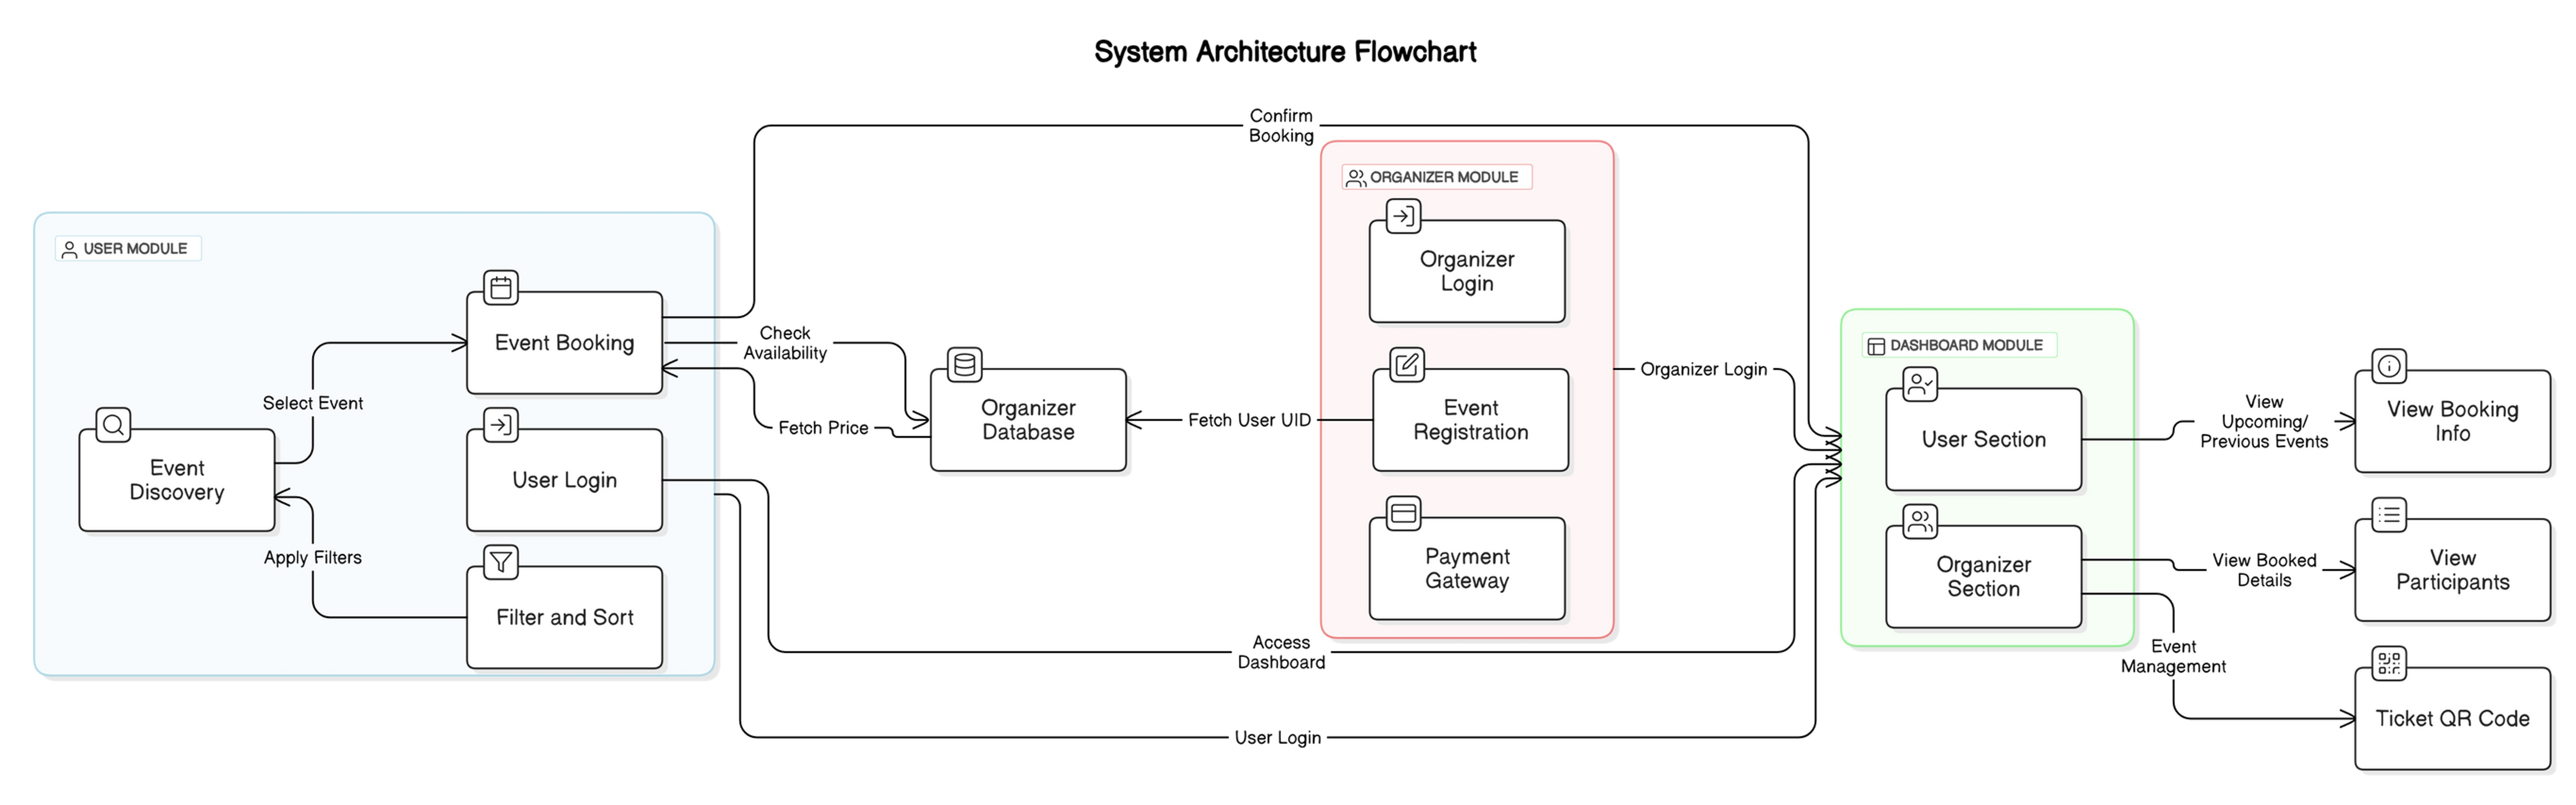
\includegraphics[scale=0.38]{system.JPG}
	\caption{\textit{System Architecture}}
	\label{fig:SystemArchitecture}
\end{figure}











\chapter{System Design}
\section { Design Diagrams }
\subsection{Use Case Diagram}
\begin{figure}[H]
	\centering
	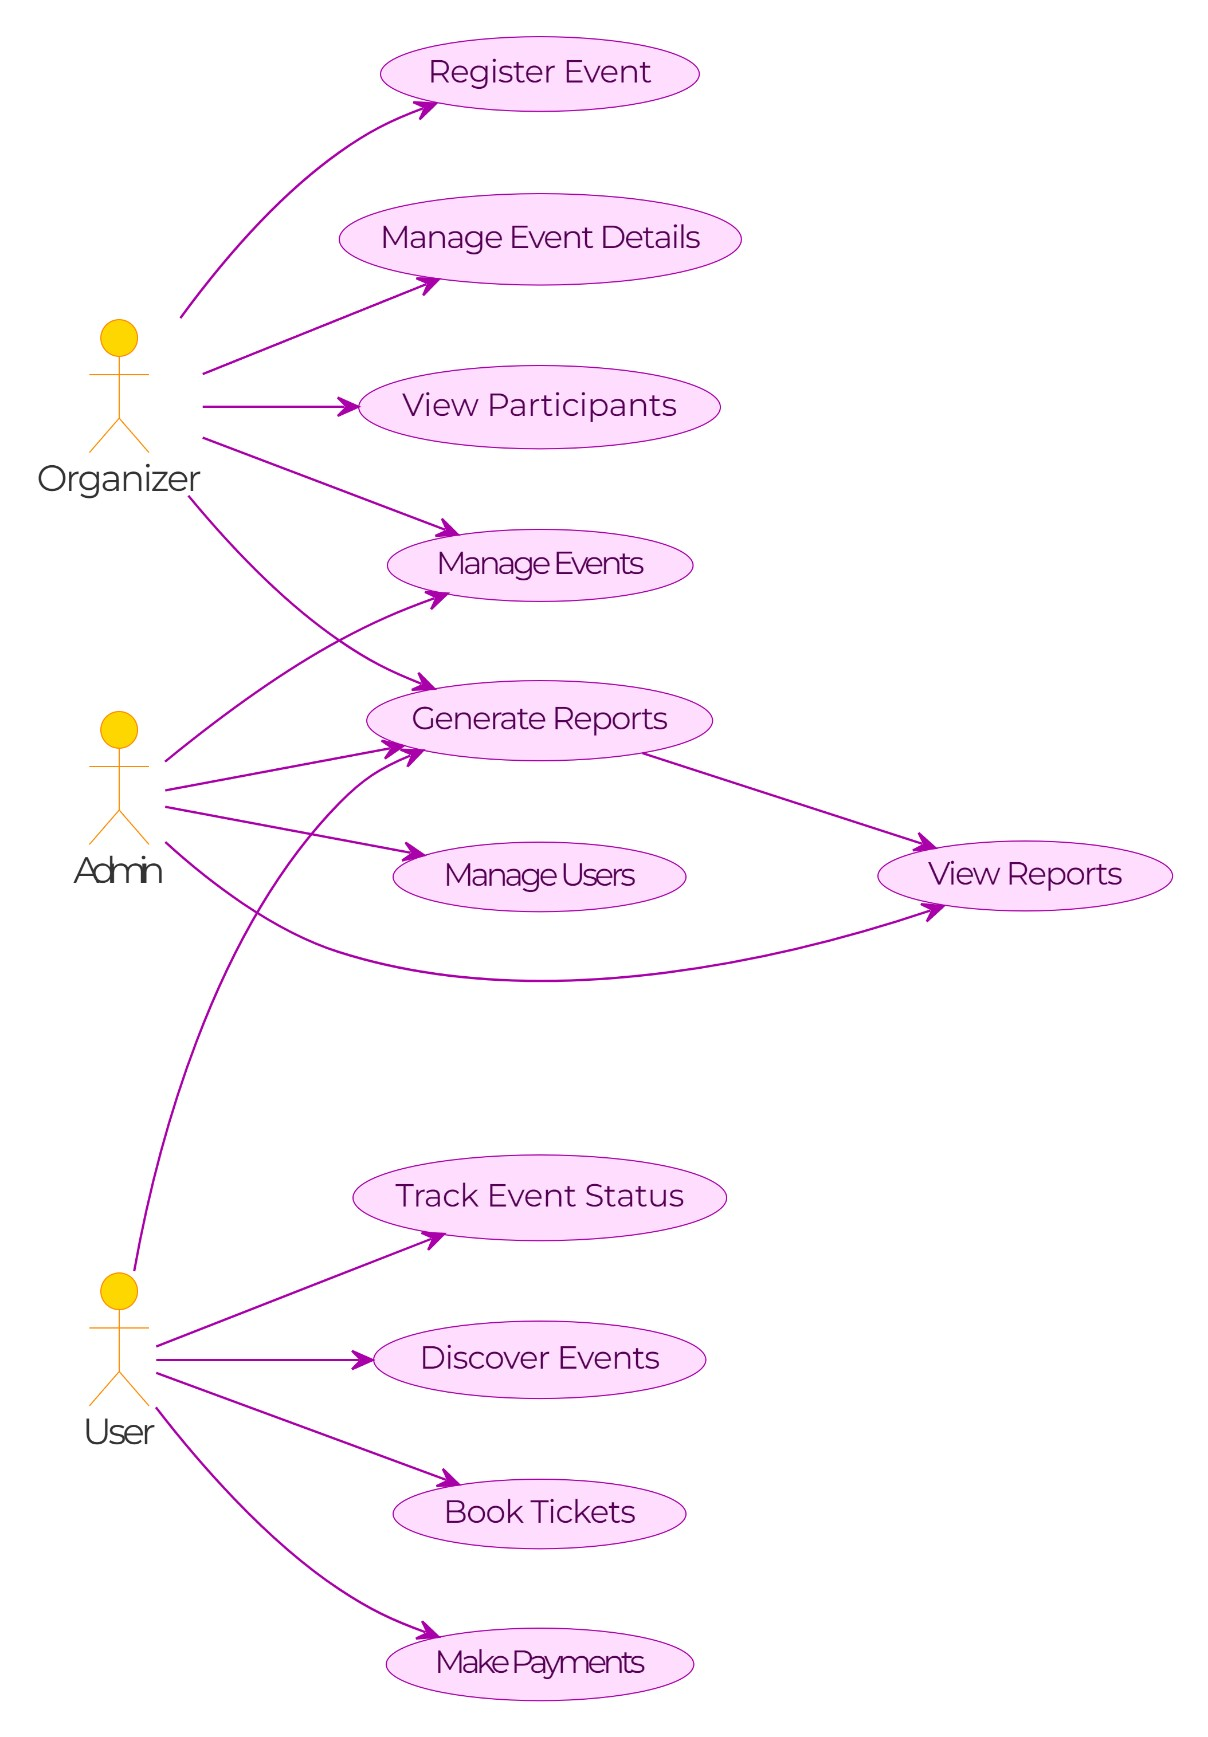
\includegraphics[scale=0.50]{use.jpg}   
	\caption{\textit{Use Case diagram}}
	\label{fig:use-case-diagram}
\end{figure}


\subsection{Sequence Diagram}
%\setcounter{figure}{1}
%\renewcommand\thefigure{\thesection.\arabic{figure}}
\begin{figure}[H]
	\centering
	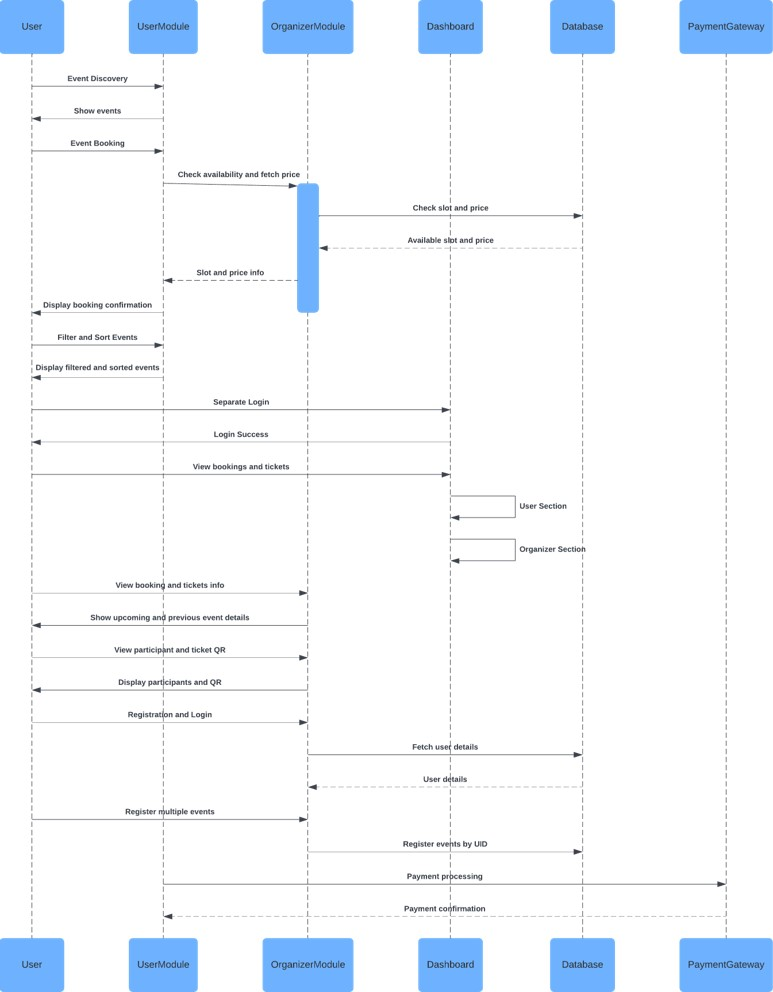
\includegraphics[scale=0.50]{sequence.jpg}   
	\caption{\textit{Sequence Diagram}}
	\label{Sequence Diagram}    
\end{figure}


%\renewcommand\thefigure{\thesection.\arabic{figure}}
\begin{figure}[H]
	%\centering
	\subsection{Data Flow Diagram}
	\hspace{2cm}
	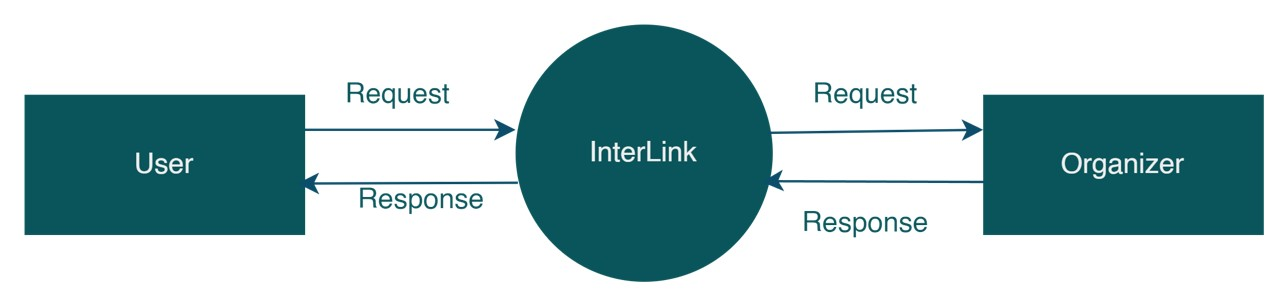
\includegraphics[width=\textwidth]{dfd1.jpg}
	\caption{\textit{LEVEL 0}}
\end{figure}

\begin{figure}[H]
	\centering
	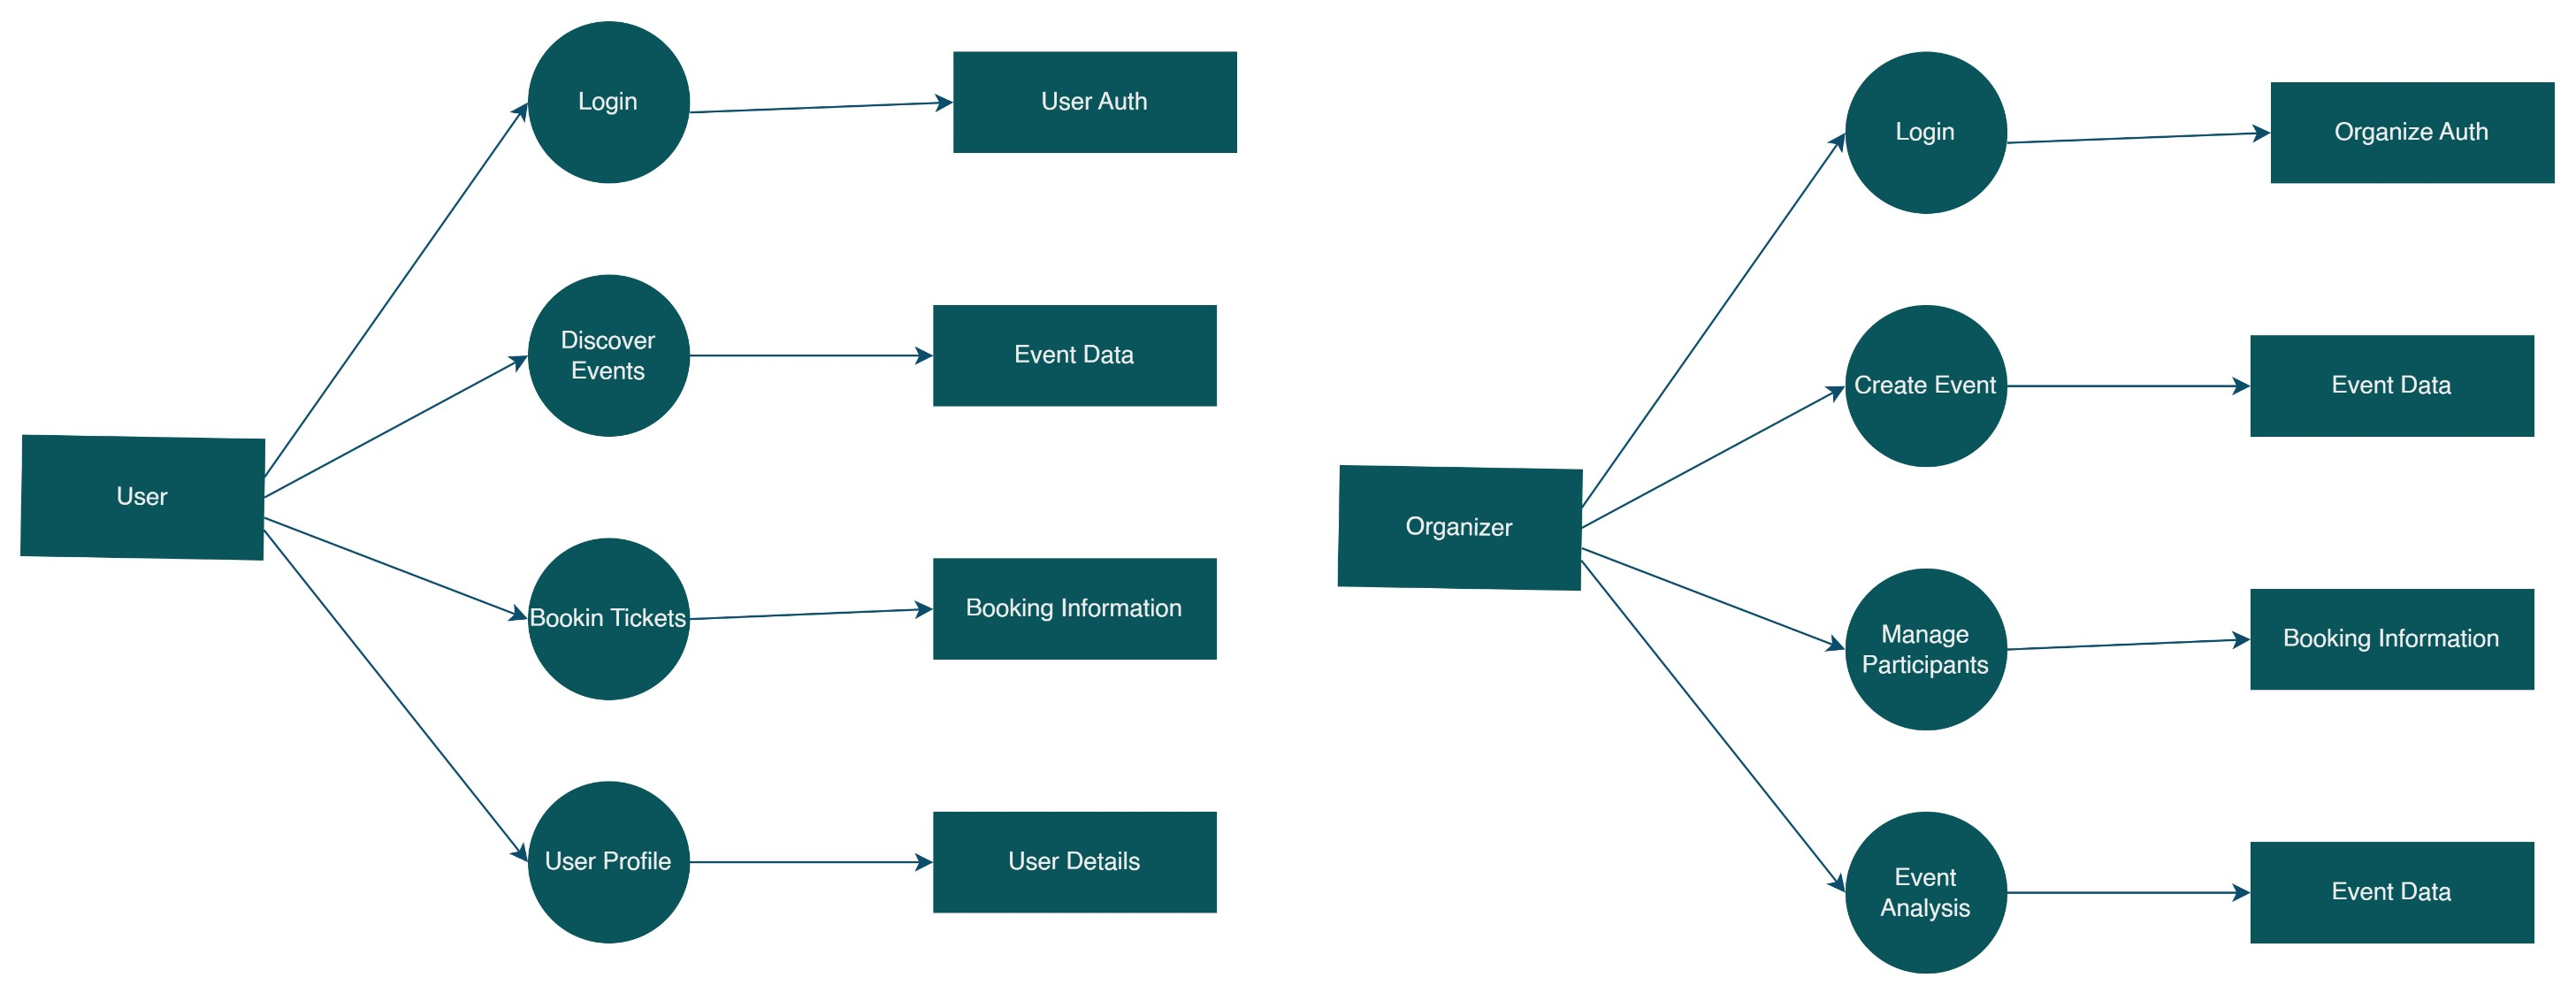
\includegraphics[scale=0.50]{dfd2.jpg}
	\caption{\textit{LEVEL 1 }}
\end{figure} 

\begin{figure}[H]
	\centering
	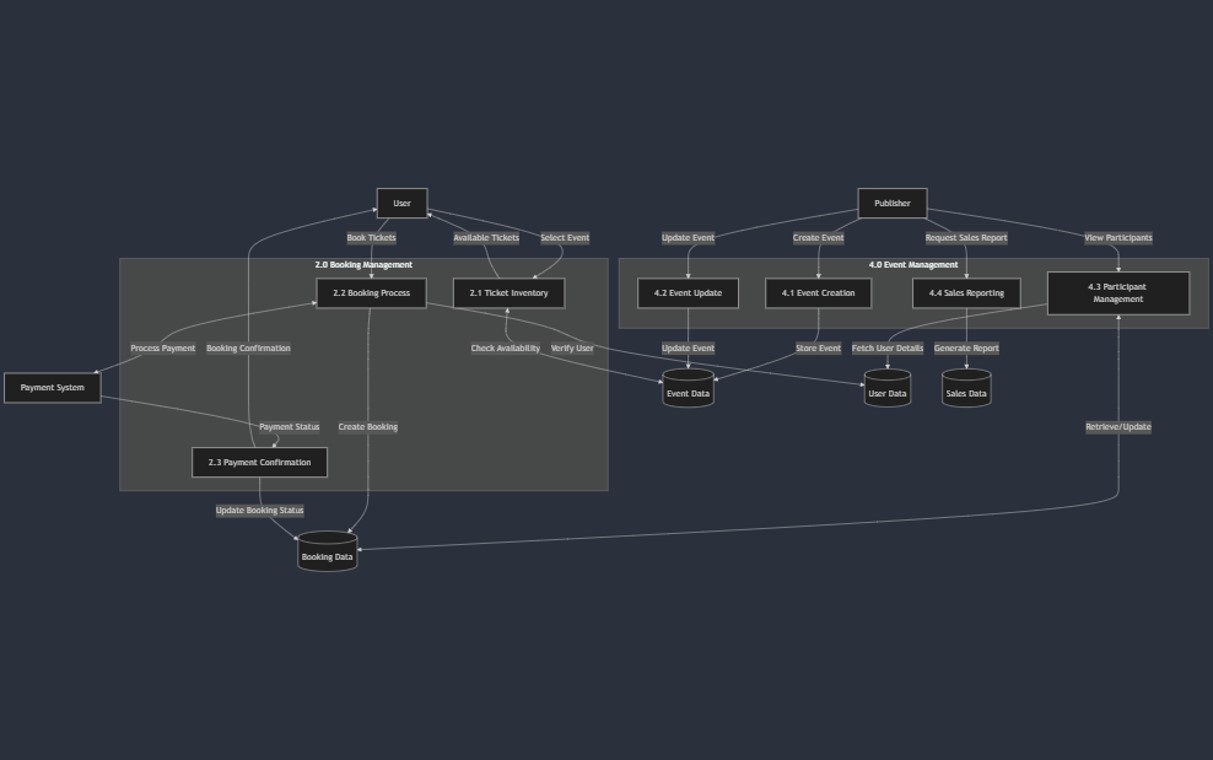
\includegraphics[width=\textwidth]{dfd3.jpg}
	\caption{\textit{LEVEL 2}}
\end{figure}  
\subsection{Activity diagram}
\begin{figure}[H]
	\centering
	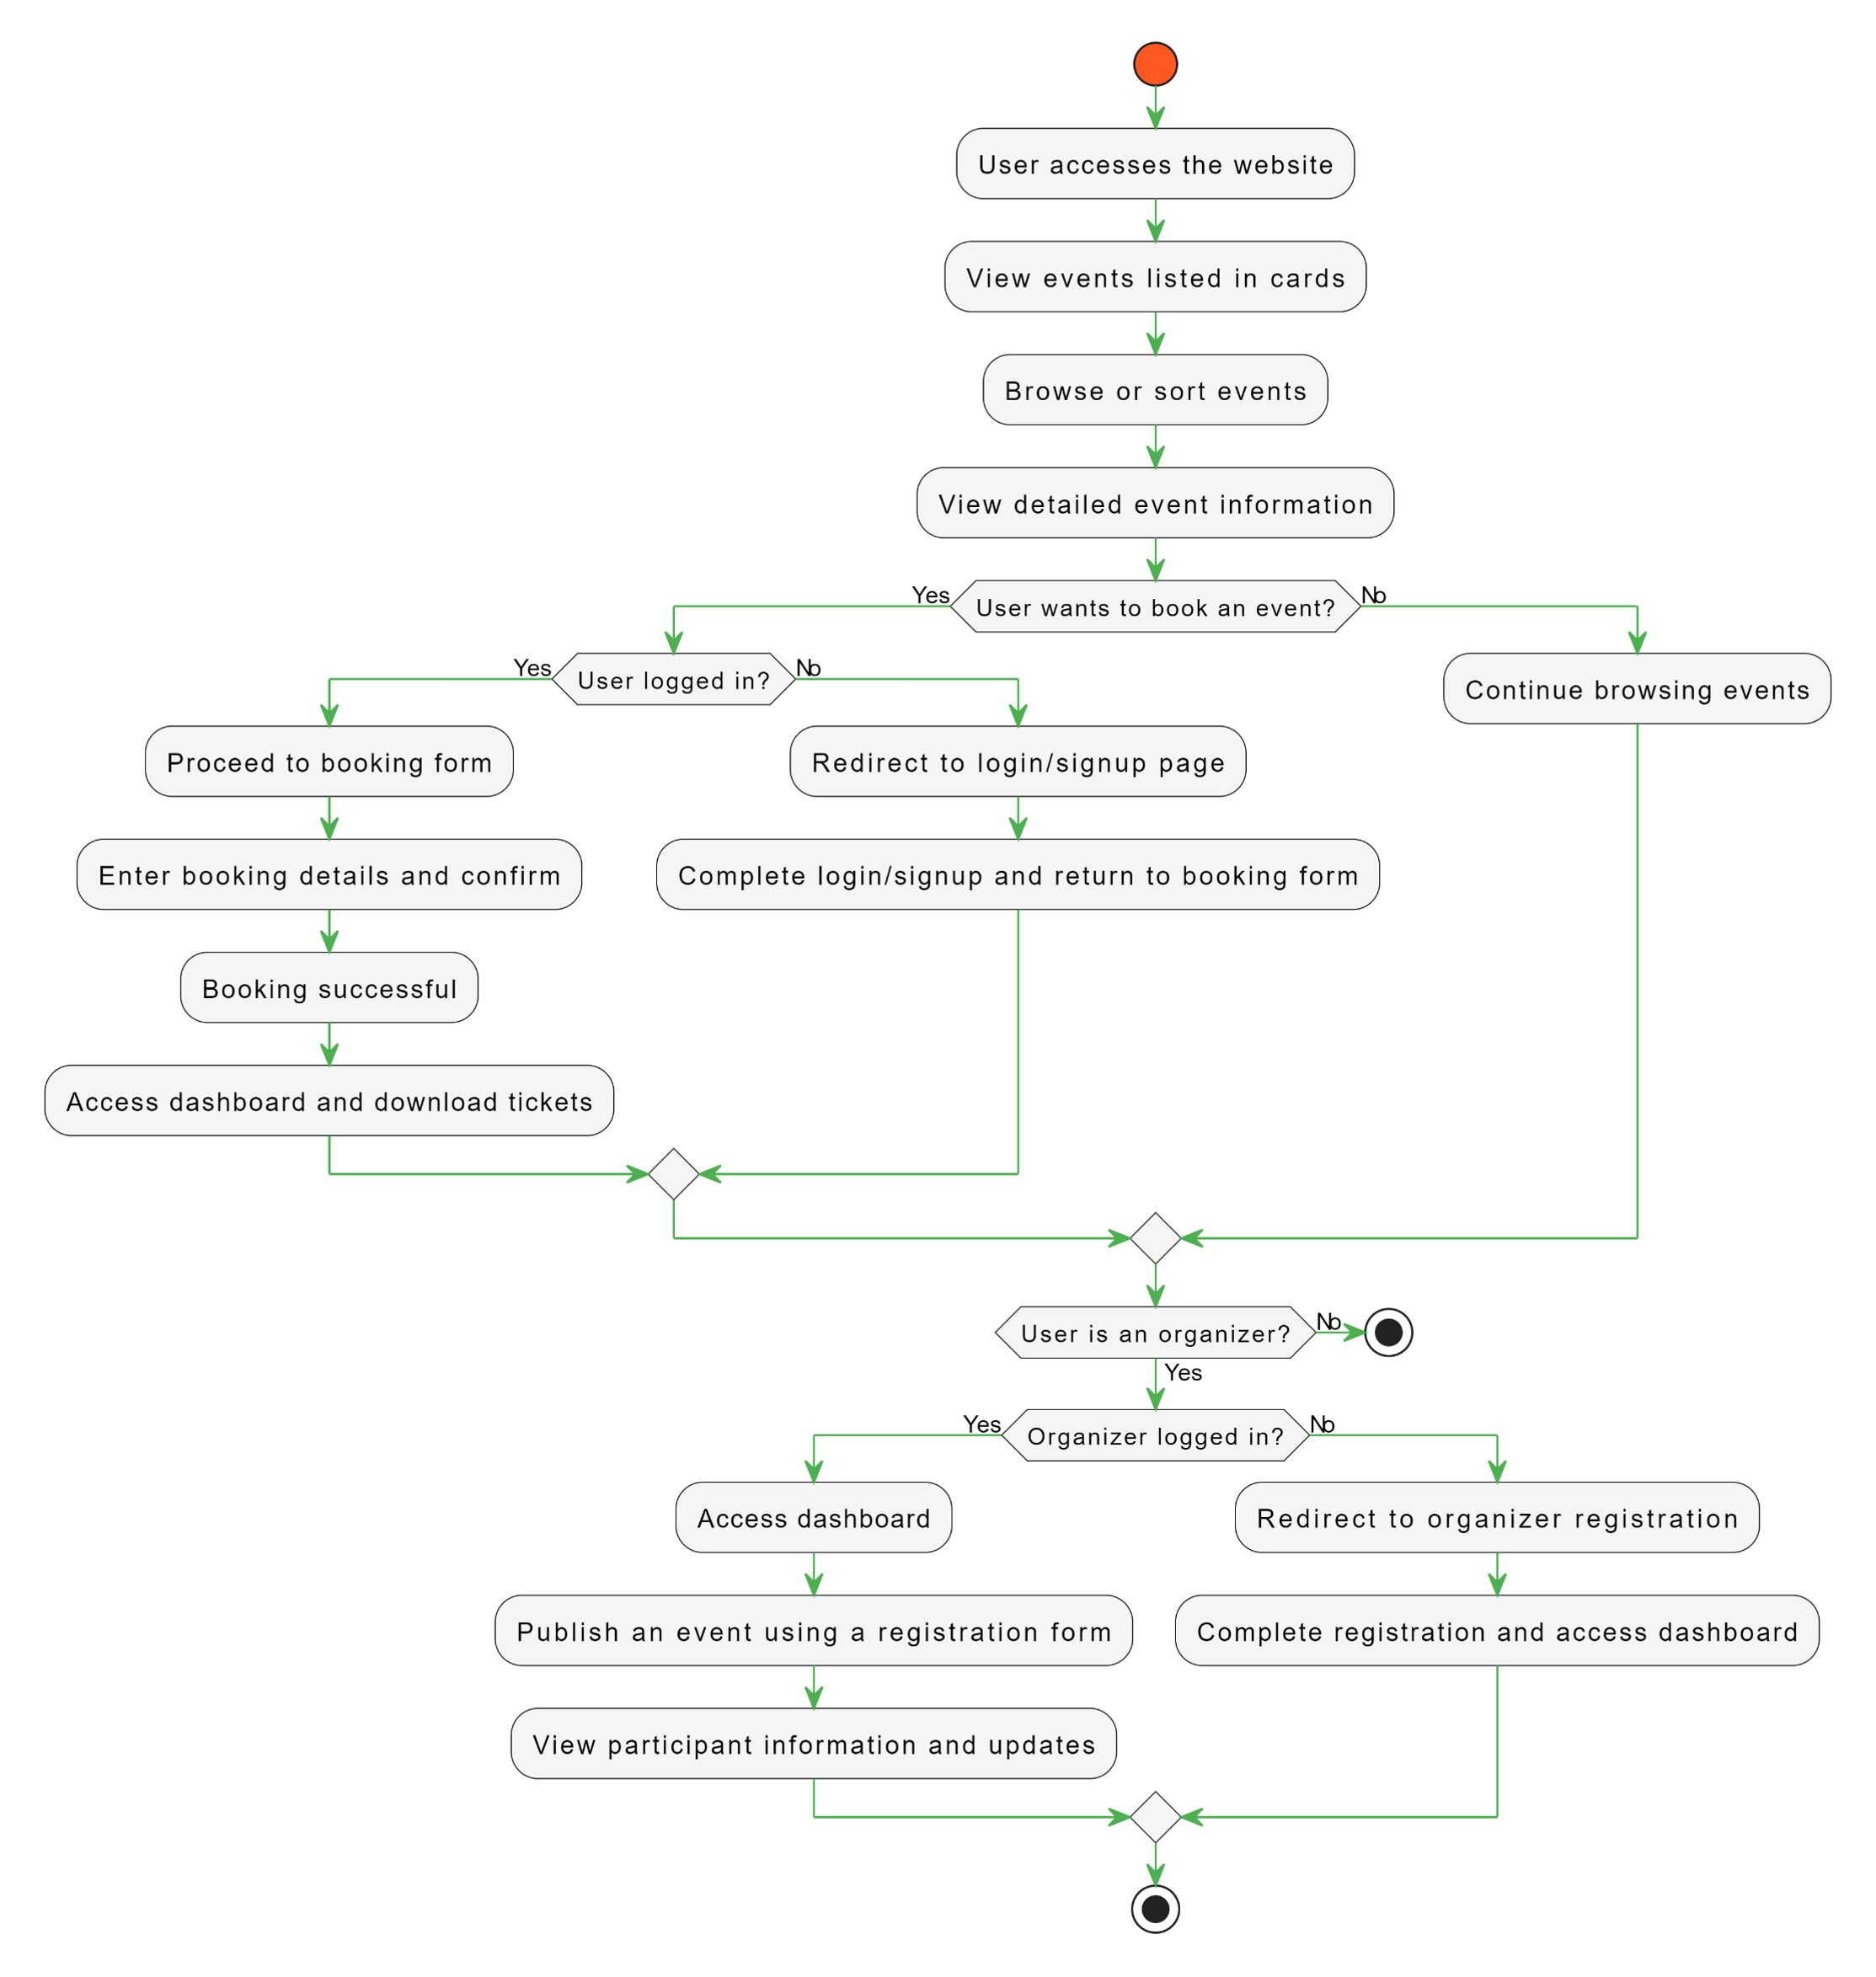
\includegraphics[scale=0.60]{activity.jpg}   
	\vspace{48pt}  % Adjust this value to reduce the space between the figure and caption
	\caption{\textit{Activity diagram}}
		\vspace{48pt}
	\label{fig:activity-diagram}
\end{figure}

\subsection{Class diagram}
\begin{figure}[H]
	\centering
	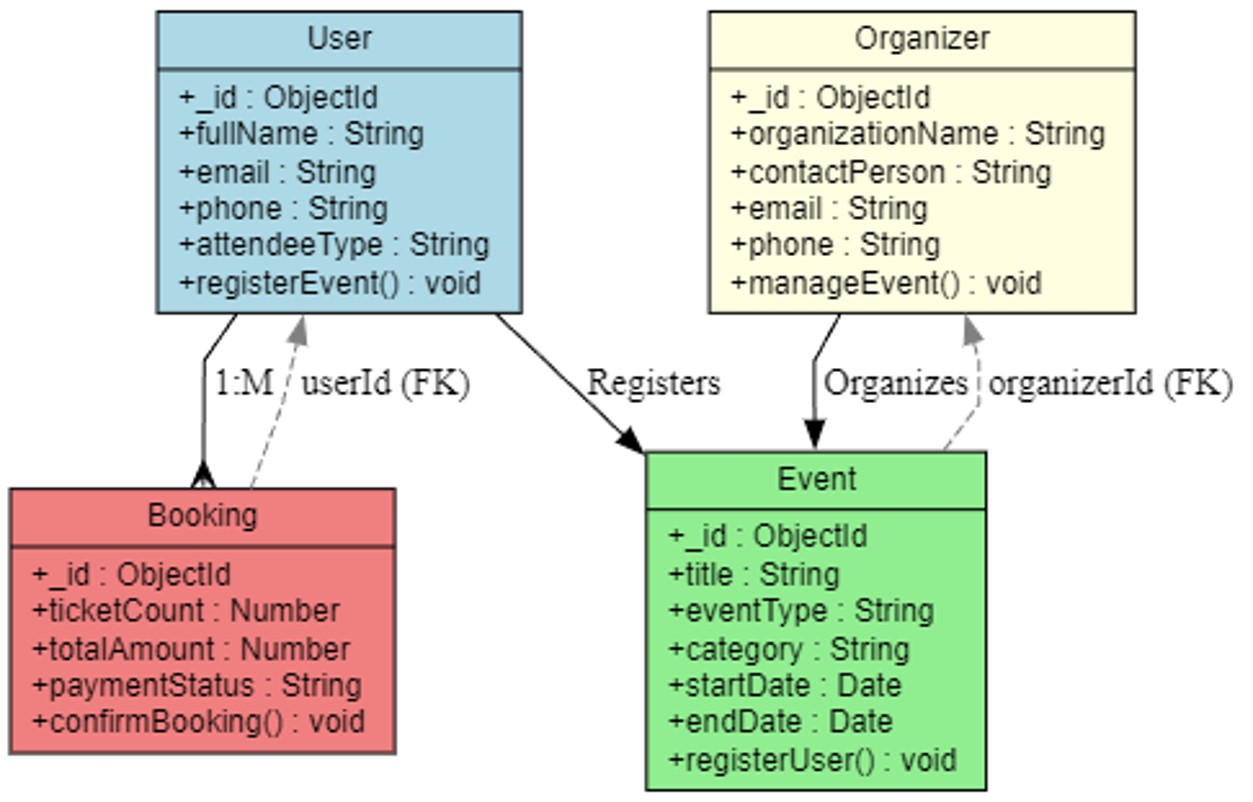
\includegraphics[scale=0.50]{class.jpg}   
	\caption{\textit{Class diagram}}
	\label{fig:class-diagram}
\end{figure}
\iffalse
\subsection{Sequential Diagram}
\begin{figure}[H]
	\centering
	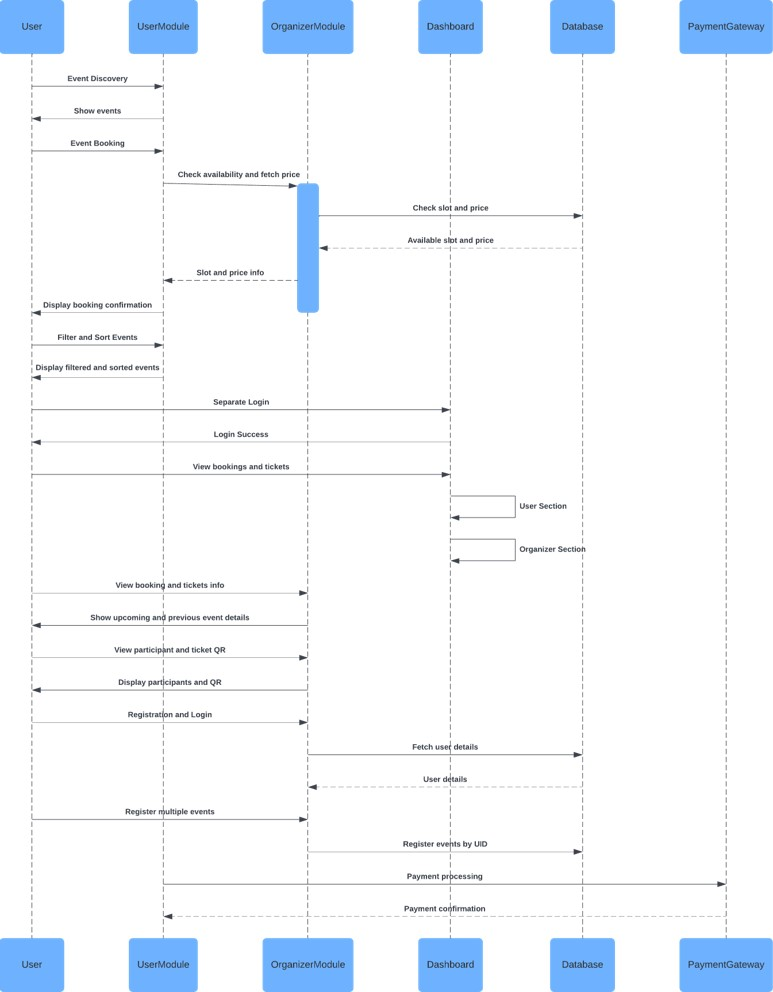
\includegraphics[scale=0.35]{sequence.jpg}  
	\caption{\textit{Sequence}}
	\label{fig:sequential-diagram}
\end{figure}

\subsection{Data Flow Diagram}
\begin{figure}[H]
	\centering
	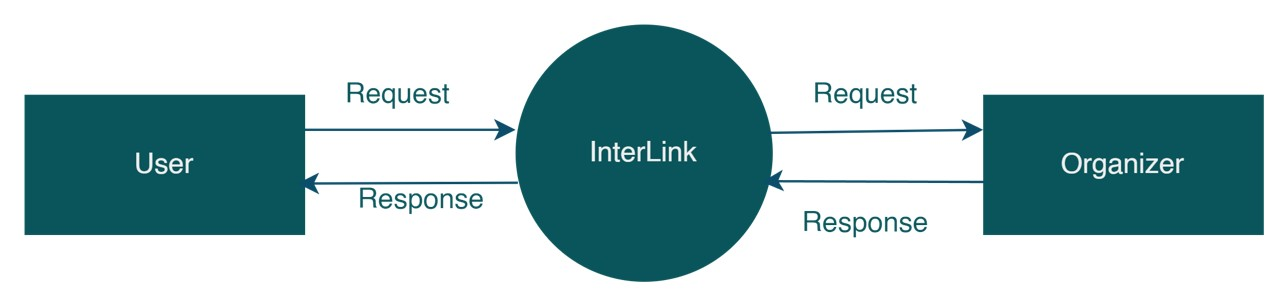
\includegraphics[width=\textwidth]{dfd1.jpg}
	\caption{DFD Level 0}
	\label{fig:dfd0}
\end{figure}

\begin{figure}[H]
	\centering
	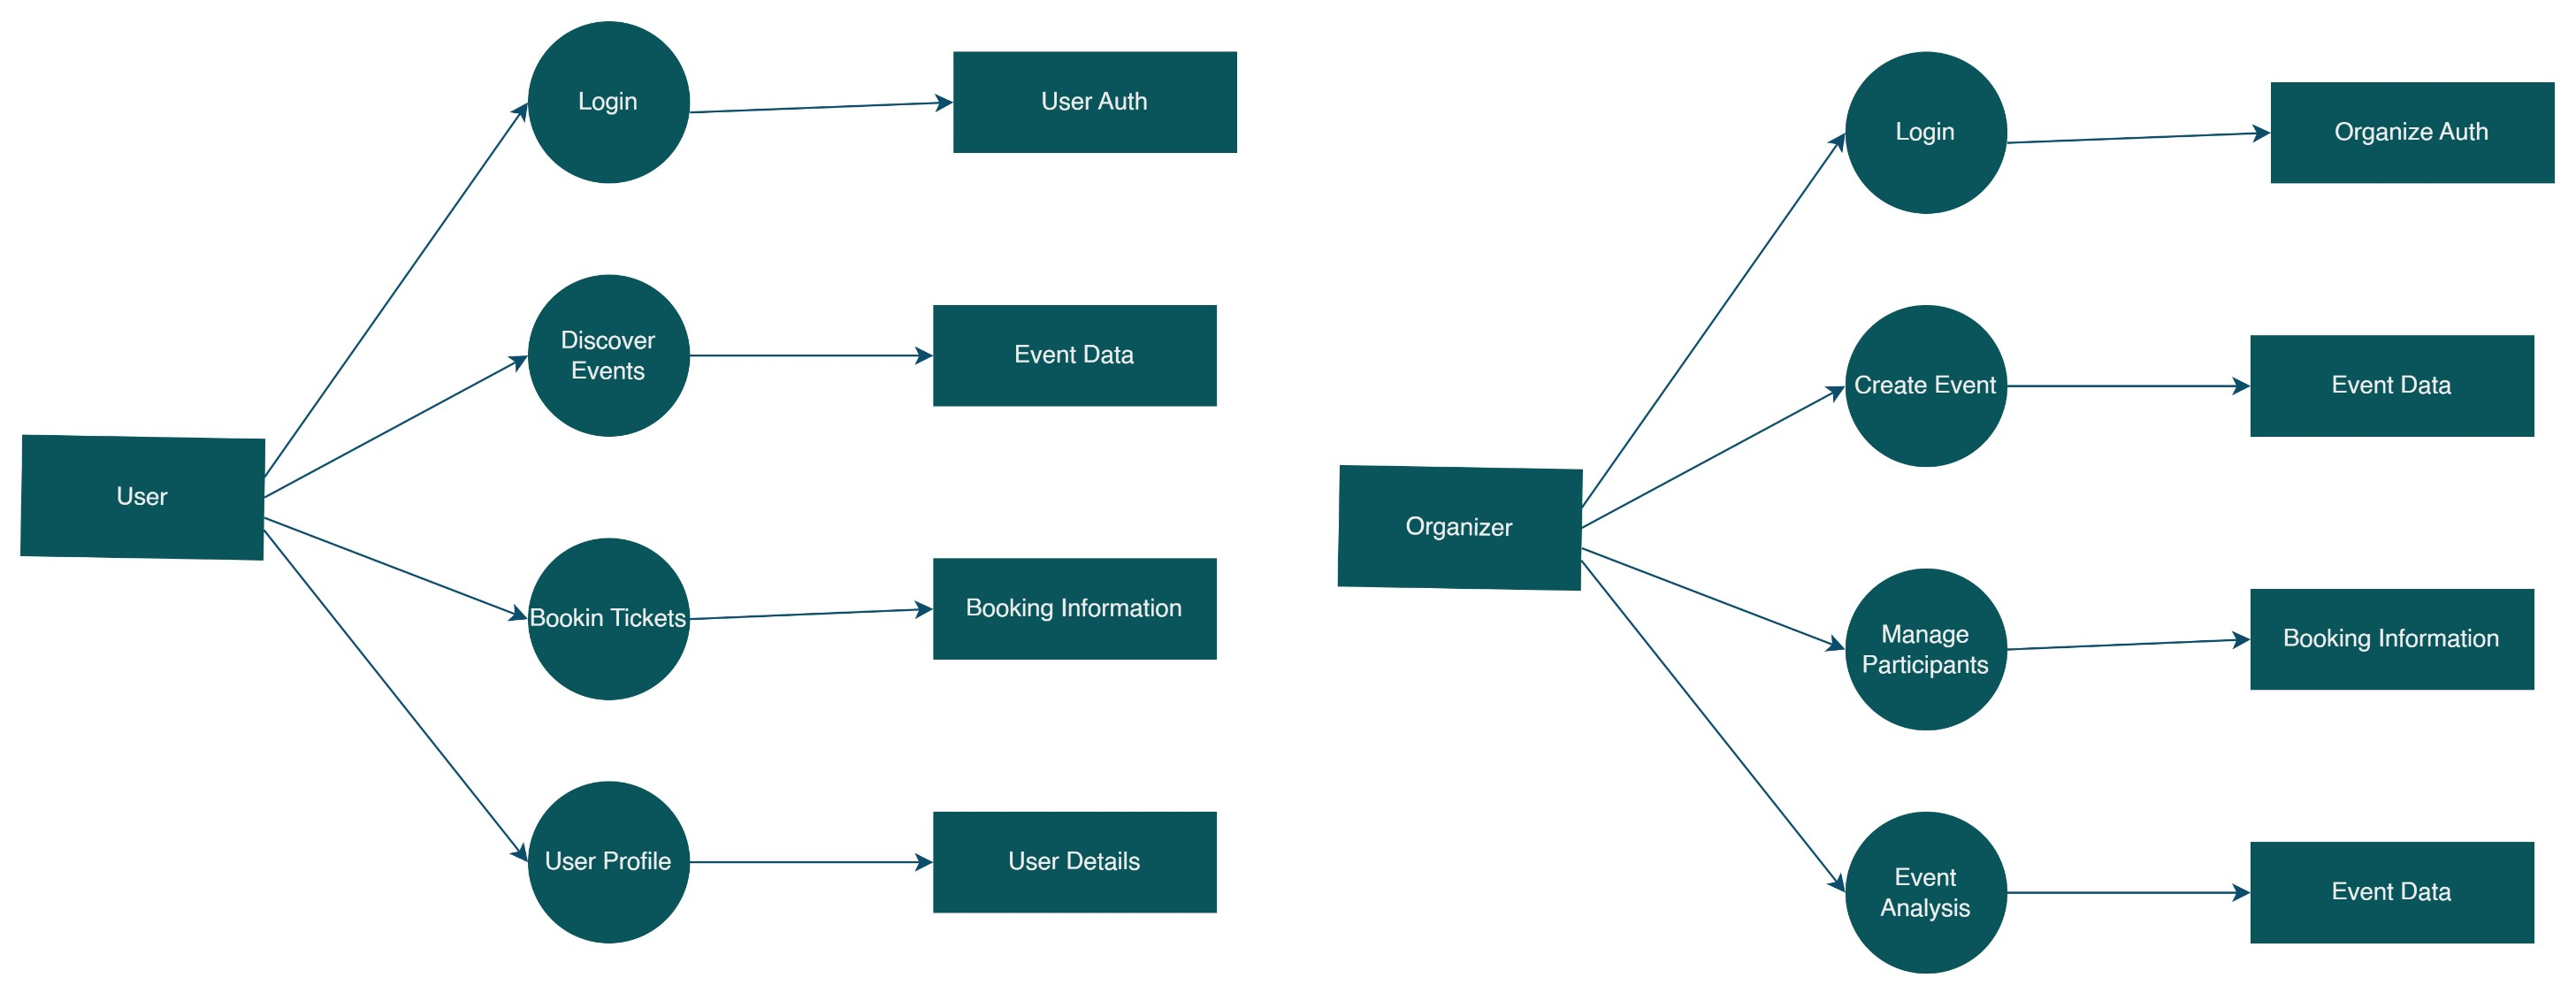
\includegraphics[width=\textwidth]{dfd2.jpg}
	\caption{DFD Level 1}
	\label{fig:dfd1}
\end{figure}

\begin{figure}[H]
	\centering
	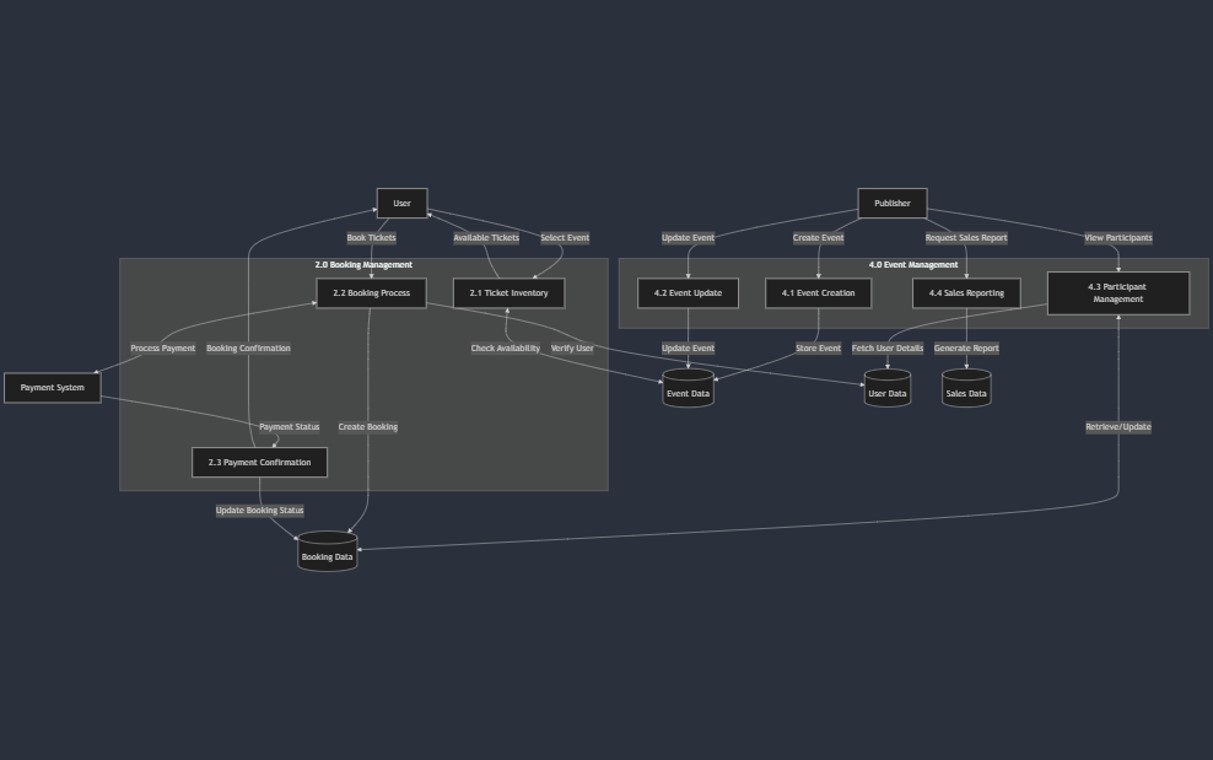
\includegraphics[width=\textwidth]{dfd3.jpg}
	\caption{DFD Level 2}
	\label{fig:dfd2}
\end{figure}
\fi
\newpage
\section{Functional and Nonfunctional Requirements}

\textbf{FUNCTIONAL REQUIREMENTS}

\begin{itemize}
	\item \textbf{R1: User Authentication and Management:}
	\begin{itemize}
		\item Input: Users provide registration details (email, password) or login credentials.
		\item Output: System returns a confirmation message, authentication token, or password reset link.
	\end{itemize}
	
	\item \textbf{R2: Event Listing and Management:}
	\begin{itemize}
		\item Input: Publishers input event details like title, date, venue, and ticket price.
		\item Output: Events are listed on the platform, and booking stats are updated.
	\end{itemize}
	
	\item \textbf{R3: Dashboard and Notifications:}
	\begin{itemize}
		\item Input: Users perform actions like booking, cancellations, or event creation.
		\item Output: Dashboards display relevant information, and notifications are sent for updates.
	\end{itemize}
	
	\item \textbf{R4: Event Search and Filtering:}
	\begin{itemize}
		\item Input: Users enter search queries or select filters like event type, location, or date.
		\item Output: The platform displays events that match the search criteria or filter settings.
	\end{itemize}
	
	\item \textbf{R5: Ticket Booking and Management:}
	\begin{itemize}
		\item Input: Users provide booking details, including the number of tickets and payment information.
		\item Output: Confirmation of ticket booking or cancellation, and payment status.
	\end{itemize}
	
	\item \textbf{R6: Event Validation and Verification:}
	\begin{itemize}
		\item Input: Publishers submit event details for validation and verification.
		\item Output: Event is either approved or rejected, and a notification is sent to the publisher.
	\end{itemize}
	
	\item \textbf{R7: Event Updates and Notifications:}
	\begin{itemize}
		\item Input: Publishers modify event details, such as date or cancellation.
		\item Output: Users receive notifications about the changes to the event.
	\end{itemize}
	
	\item \textbf{R8: Security Features:}
	\begin{itemize}
		\item Input: Users provide personal, registration, or payment details.
		\item Output: Data is encrypted and securely stored; transactions are processed securely.
	\end{itemize}
	
	\item \textbf{R9: Performance and Scalability:}
	\begin{itemize}
		\item Input: Increased user traffic and event data.
		\item Output: The platform maintains performance and scales to handle the load effectively.
	\end{itemize}
	
	\item \textbf{R10: Compliance and Accessibility:}
	\begin{itemize}
		\item Input: Users interact with the platform, and accessibility settings are applied.
		\item Output: The platform meets legal compliance standards and is accessible to all users.
	\end{itemize}
	
\end{itemize}

\textbf{NON-FUNCTIONAL REQUIREMENTS}

\vspace{0.5cm} % Adjust the value to increase or decrease the space

\textbf{Performance:} The website must load within 3 seconds to ensure a fast and smooth user         experience. 

\textbf{Scalability:} The platform should be able to handle increased user traffic and event data without
performance issues.

\textbf{Reliability:} The website should operate reliably under normal conditions, with minimal errors      and downtime. 

\textbf{Maintainability:} The system should be easy to maintain and update, with a modular codebase
and clear documentation.

\textbf{Interoperability:} The platform should integrate seamlessly with third-party services like payment
gateways, social media, and email platforms.

\textbf{Compatibility:} Works on all browsers and devices.


\section{Hardware and Software Requirements}
%\hspace{0.5cm}
\textbf{SOFTWARE REQUIREMENTS}

\begin{verbatim}
	Frontend: React.js with TypeScript & Vite 
	Styling: Tailwind CSS 
	Backend: Node.js with Express.js 
	API Handling: Axios for HTTP requests
	Database: MongoDB (Managed via MongoDB Compass) 
	Authentication: JWT & Role-Based Access Control 
	Development Tools: VS Code, GitHub, Postman(Thunder Client) 
	Package Manager: npm 
	
\end{verbatim}
\raggedright
\textbf{HARDWARE REQUIREMENTS}

\begin{verbatim}
	Client Side (Developer Machine)
	Processor: Intel i5 / Ryzen 5 or higher
	RAM: 4GB (8GB recommended)
	Storage: 50GB free (SSD preferred)
	GPU: Integrated or dedicated GPU
	Network: Stable internet for API & deployment
	
	Server Side (Hosting Environment)
	Processor: Intel i5 / Ryzen 7 or higher
	RAM: Minimum 8GB (16GB+ for scalability)
	Storage: SSD-based (50GB+ for database & files)
	Network: High-speed internet with 99.9% uptime
	OS: Linux (Ubuntu preferred)
	
\end{verbatim}
%\newpage
\section {Project Scheduling } 
 	
\begin{table}[H]
	\centering

	\caption{Project Time line}
	\begin{tabular}{|>{\centering\arraybackslash}m{3cm} |>{\centering\arraybackslash}m{6cm} |>{\centering\arraybackslash}m{5cm}|}
		\hline
		\textbf{Task } & \textbf{Task Description} & \textbf{Time Slot} \\
		\hline
		Problem Identification & Identify the specific challenges and requirements of the event publishing system. & 17/12/2024 \\
		\hline
		System Analysis & Analyze the creation process, user needs, and technical requirements. & 08/01/2025 \\
		\hline
		GUI Design &Design the user interface for the interLink platform , including layout, templates. & 18/02/2025 \\
		\hline
		Database Design  &Design the database structure and database management system. & 03/03/2025  \\
		\hline
		System Implementation &Develop the frontend using React js and backend using Node js and database using Mongo DB. & 10/03/2025\\
		\hline
		Testing and Refinement & Thoroughly test the interLink platform , identify and fix bugs, and refine user experience.& 20/03/25 \\
		\hline
		Report Preparation &  Prepare the project report, documenting the entire process, system architecture, design choices. & 03/04/25 \\
		\hline 
		Final Review  &Review the project, finalize the report, and prepare for the projects’s final review. & 04/04/25 \\
		\hline 
	\end{tabular}
	%\caption{Project Schedule}
	\label{tab:PrjctTimLin}
\end{table}
\section {GUI Design}
\begin{flushleft}
	\begin{figure}[H]
		\centering
		
		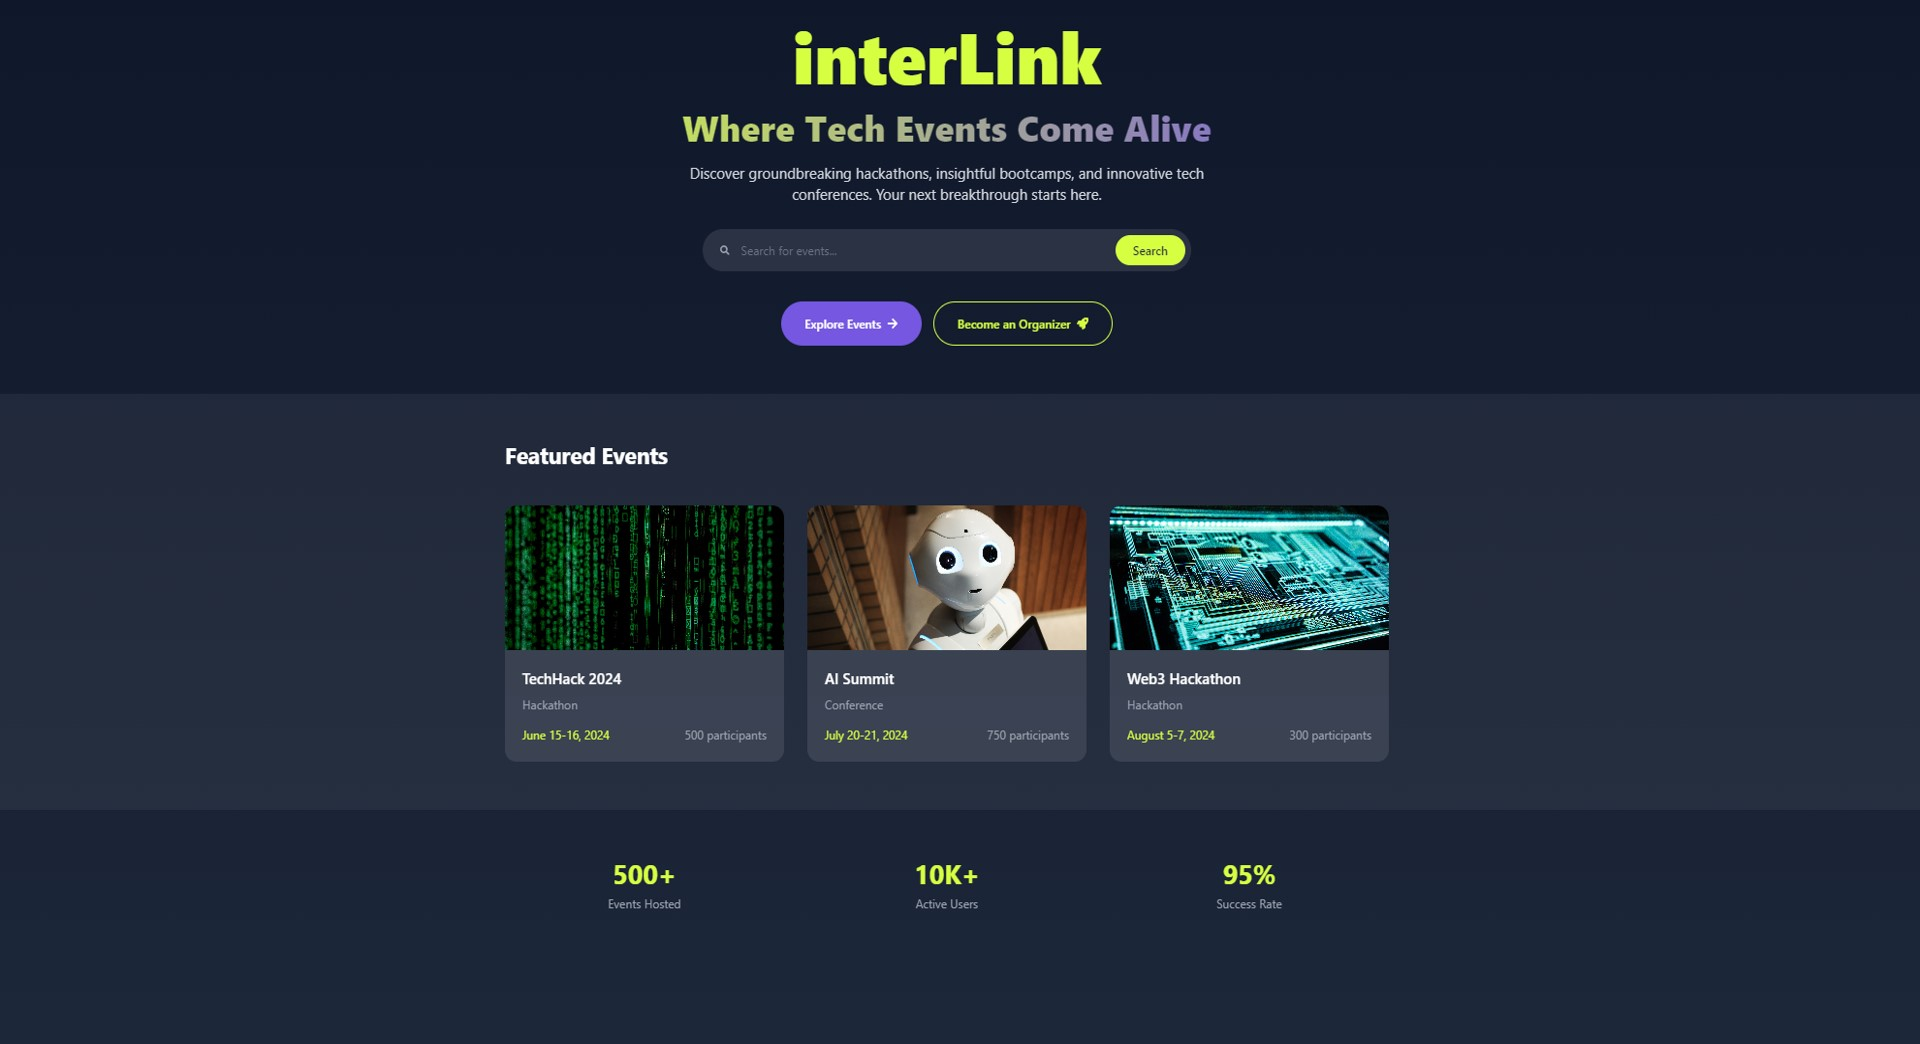
\includegraphics[scale=0.35]{r1.jpg}  
		\caption{Home Page} % Description above the image   
	\end{figure}
	
	\begin{figure}[H]
		\centering
		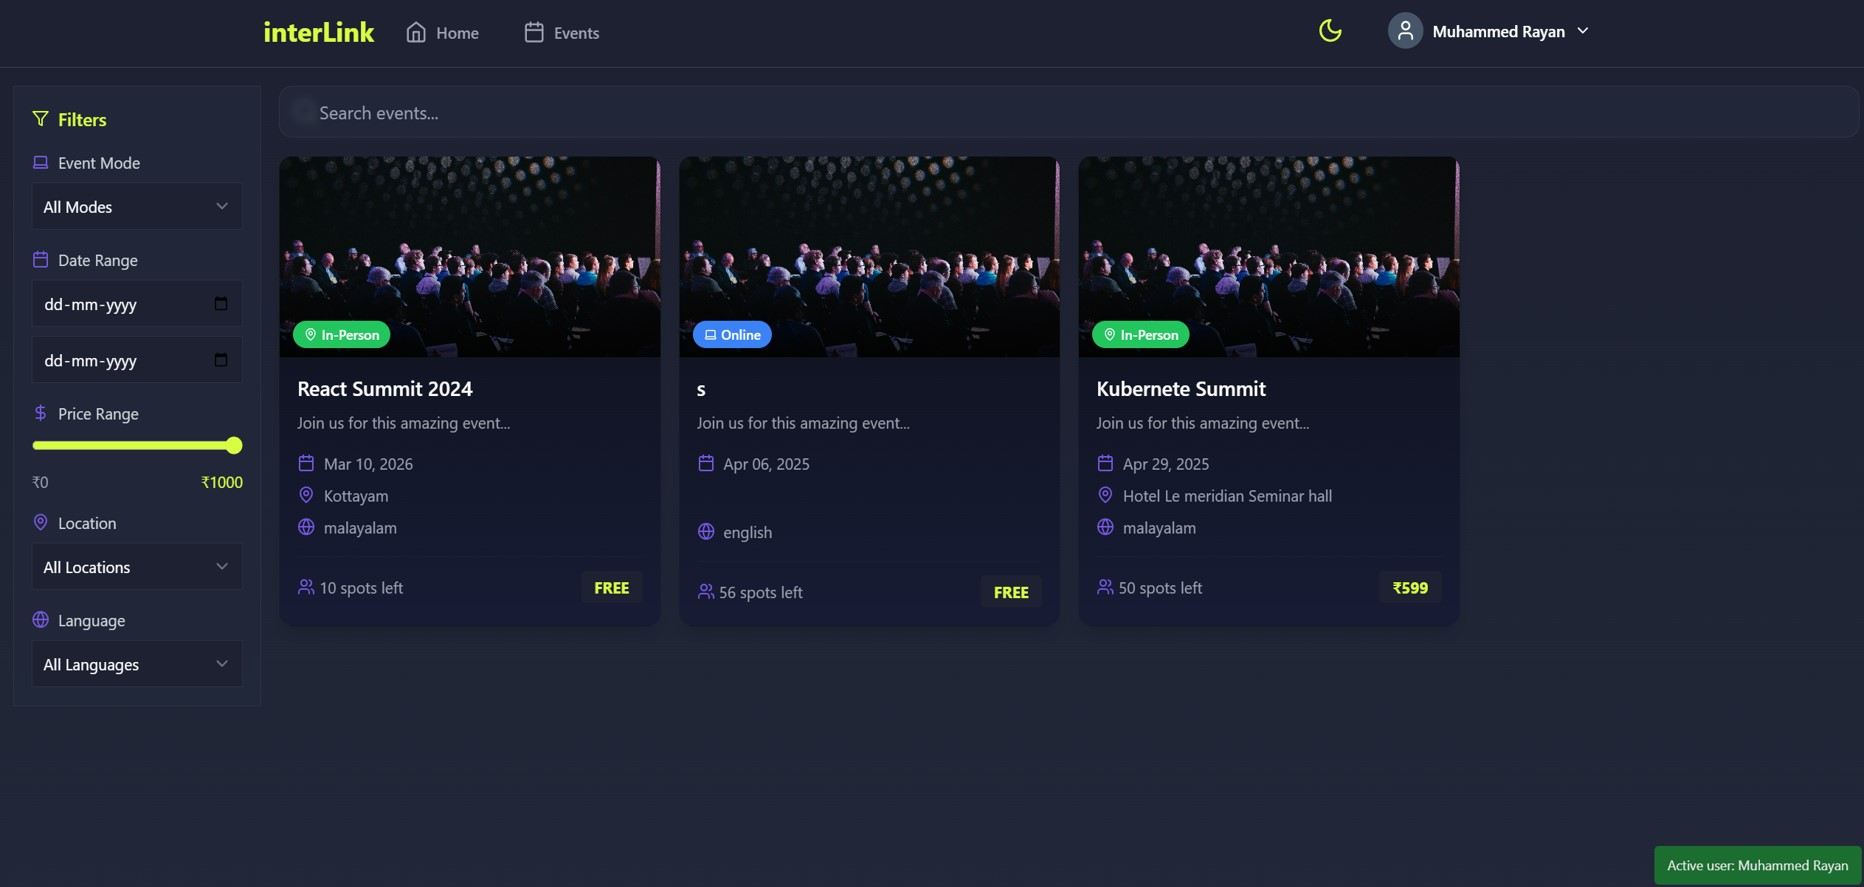
\includegraphics[scale=0.35]{r2.jpg}   
		\caption{Event Discovery} % Description above the image  
	\end{figure}
	
	\begin{figure}[H]
		\centering
		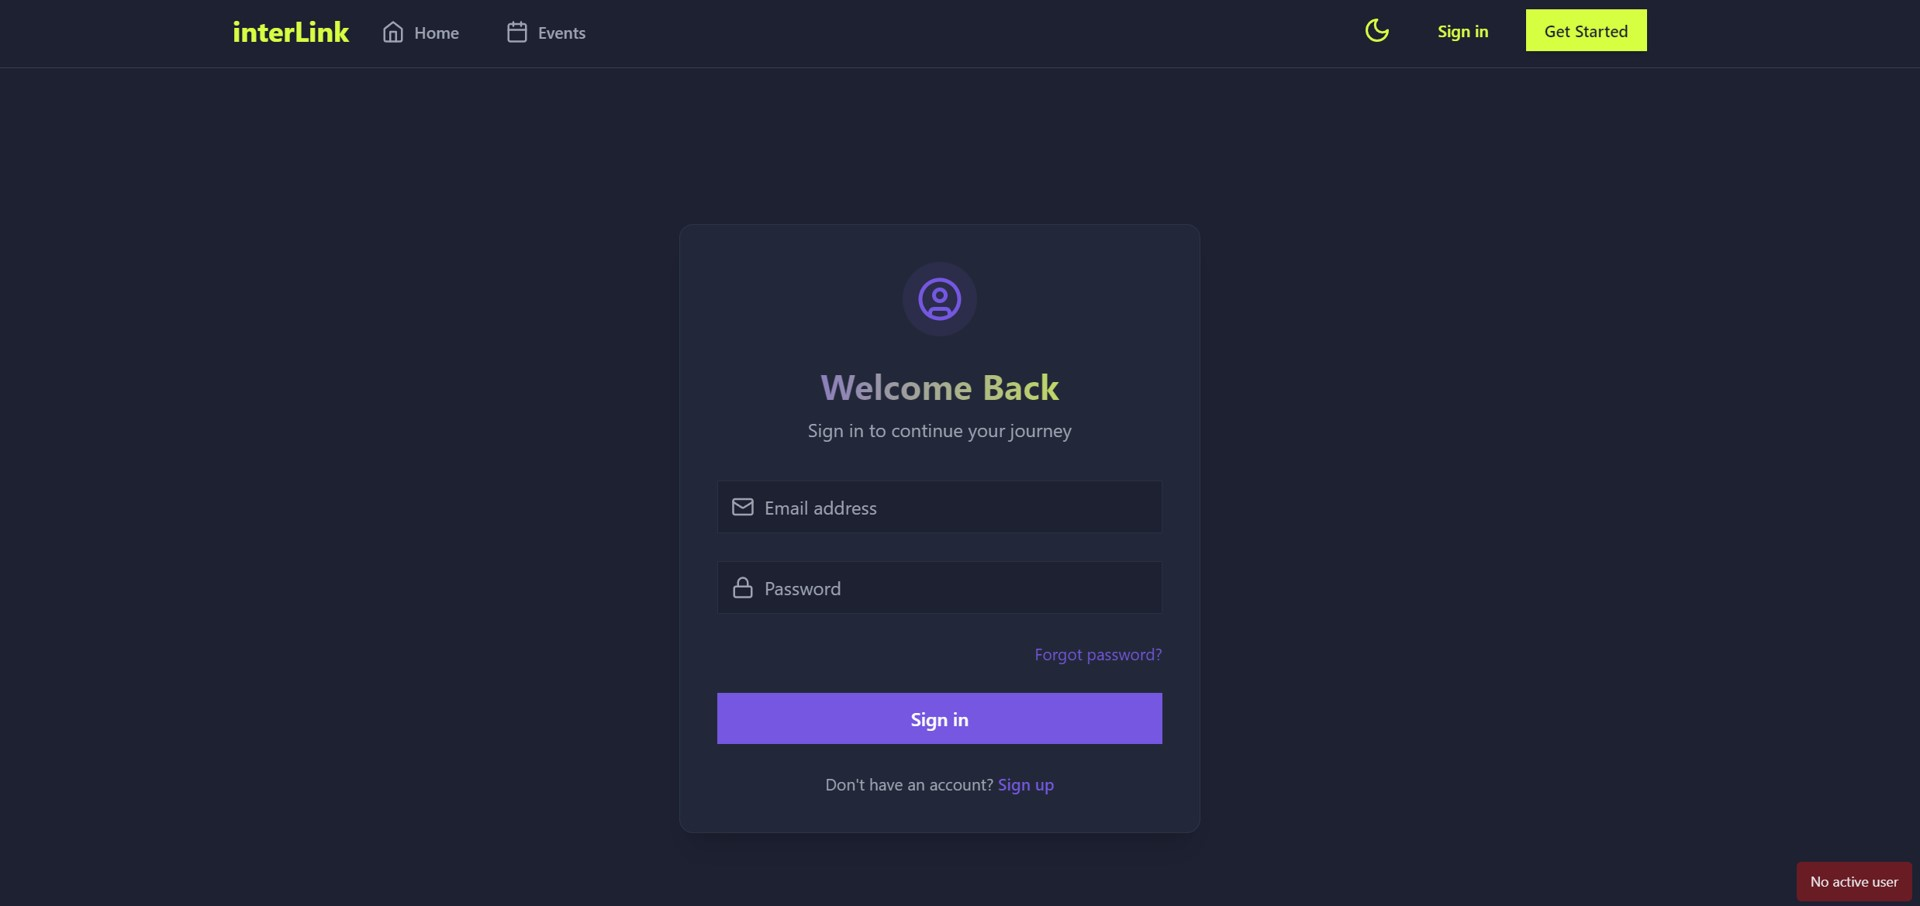
\includegraphics[scale=0.35]{r3.jpg}   
		\caption{Sign In} % Description above the image  
	\end{figure}
	
	\begin{figure}[H]
		\centering
		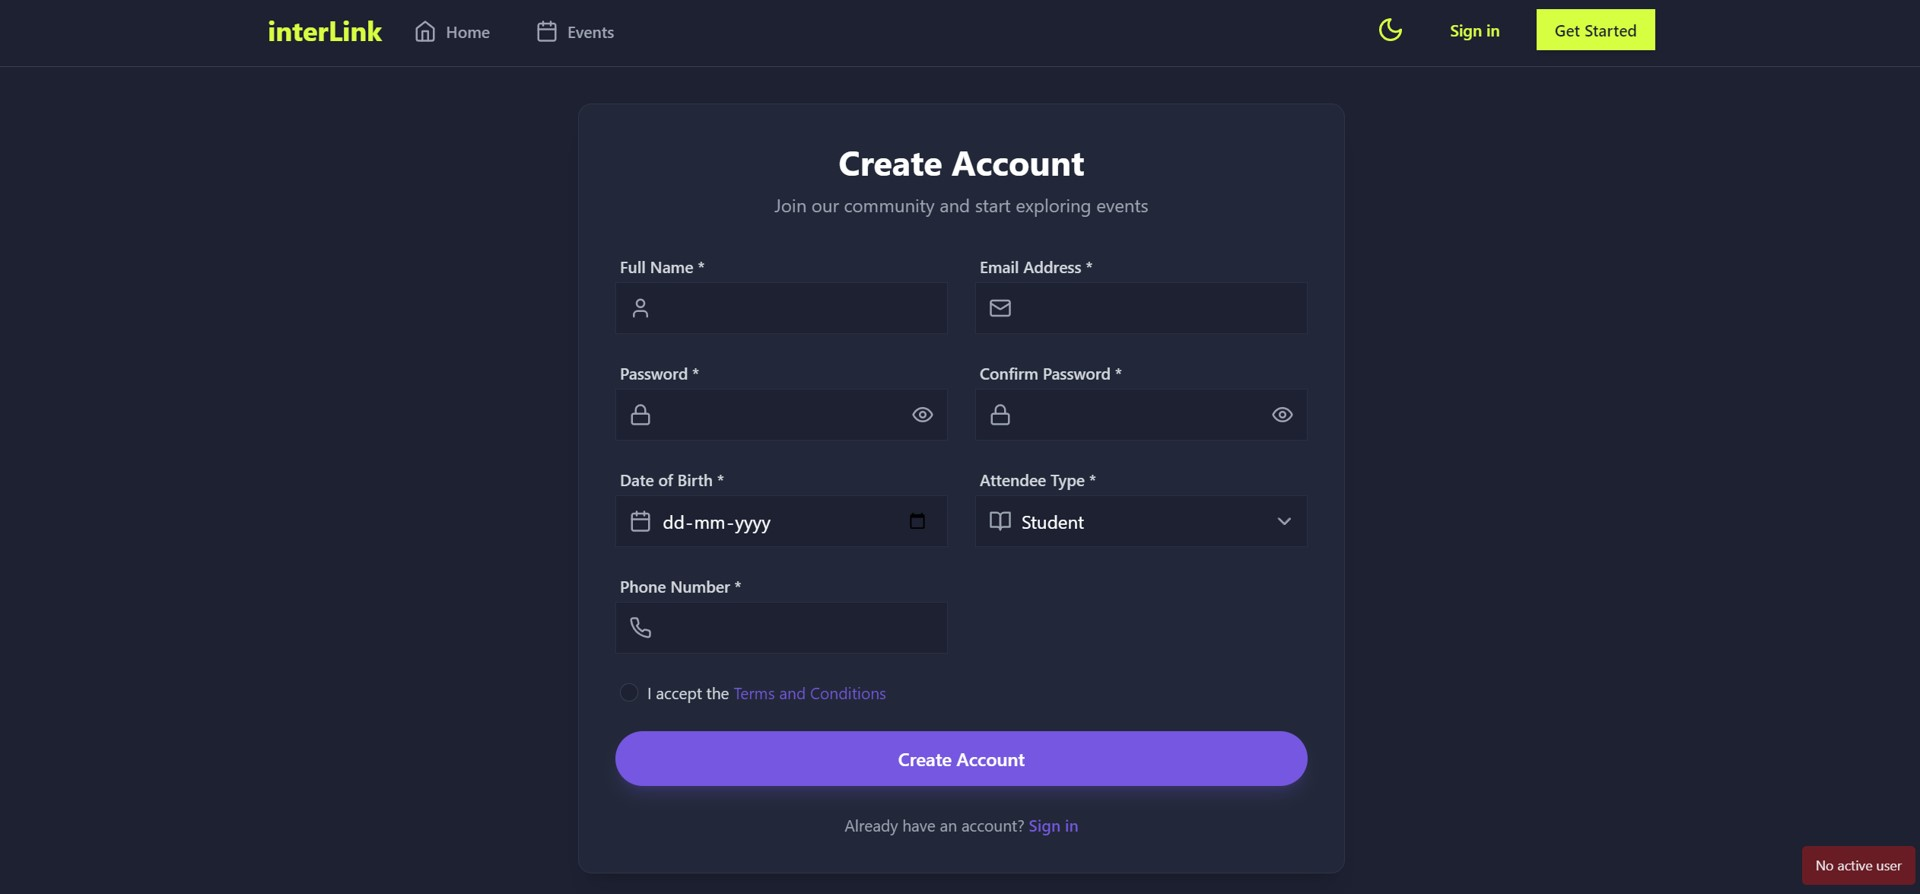
\includegraphics[scale=0.35]{r4.jpg}    
		\caption{Sign Up} % Description above the image 
	\end{figure}
	
	\begin{figure}[H]
		\centering
		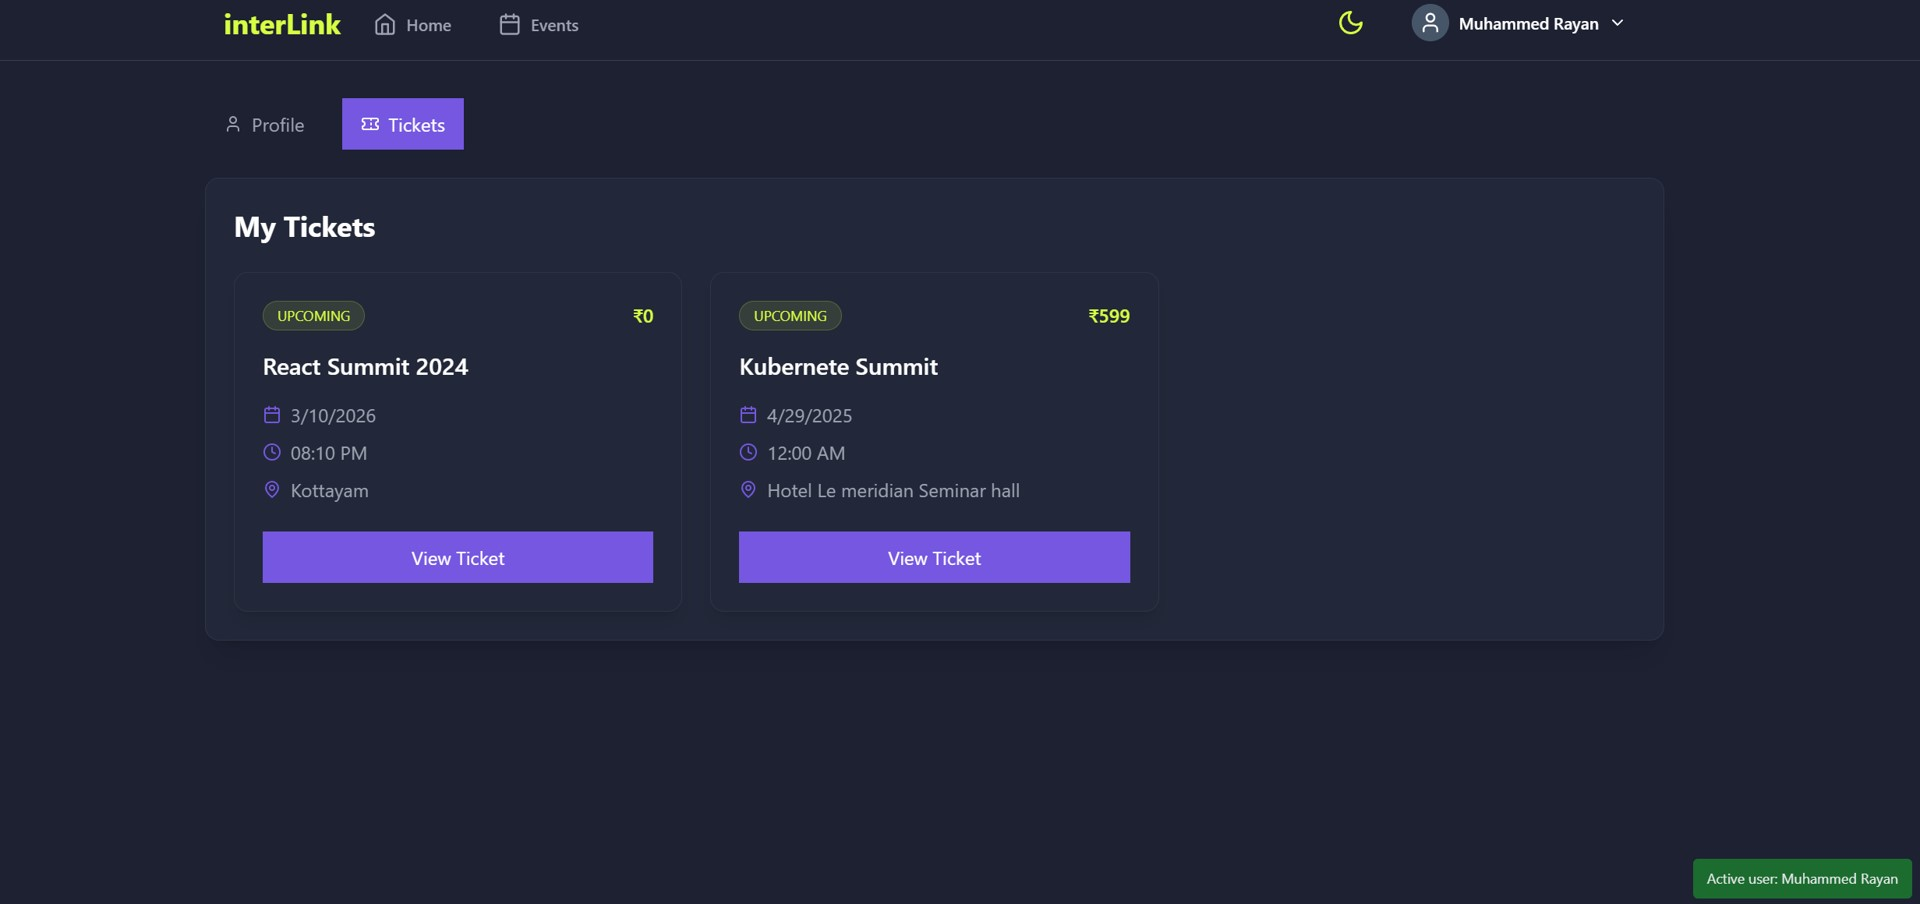
\includegraphics[scale=0.35]{r5.jpg}  
		\caption{Ticket Track} % Description above the image   
	\end{figure}
	
	\begin{figure}[H]
		\centering
		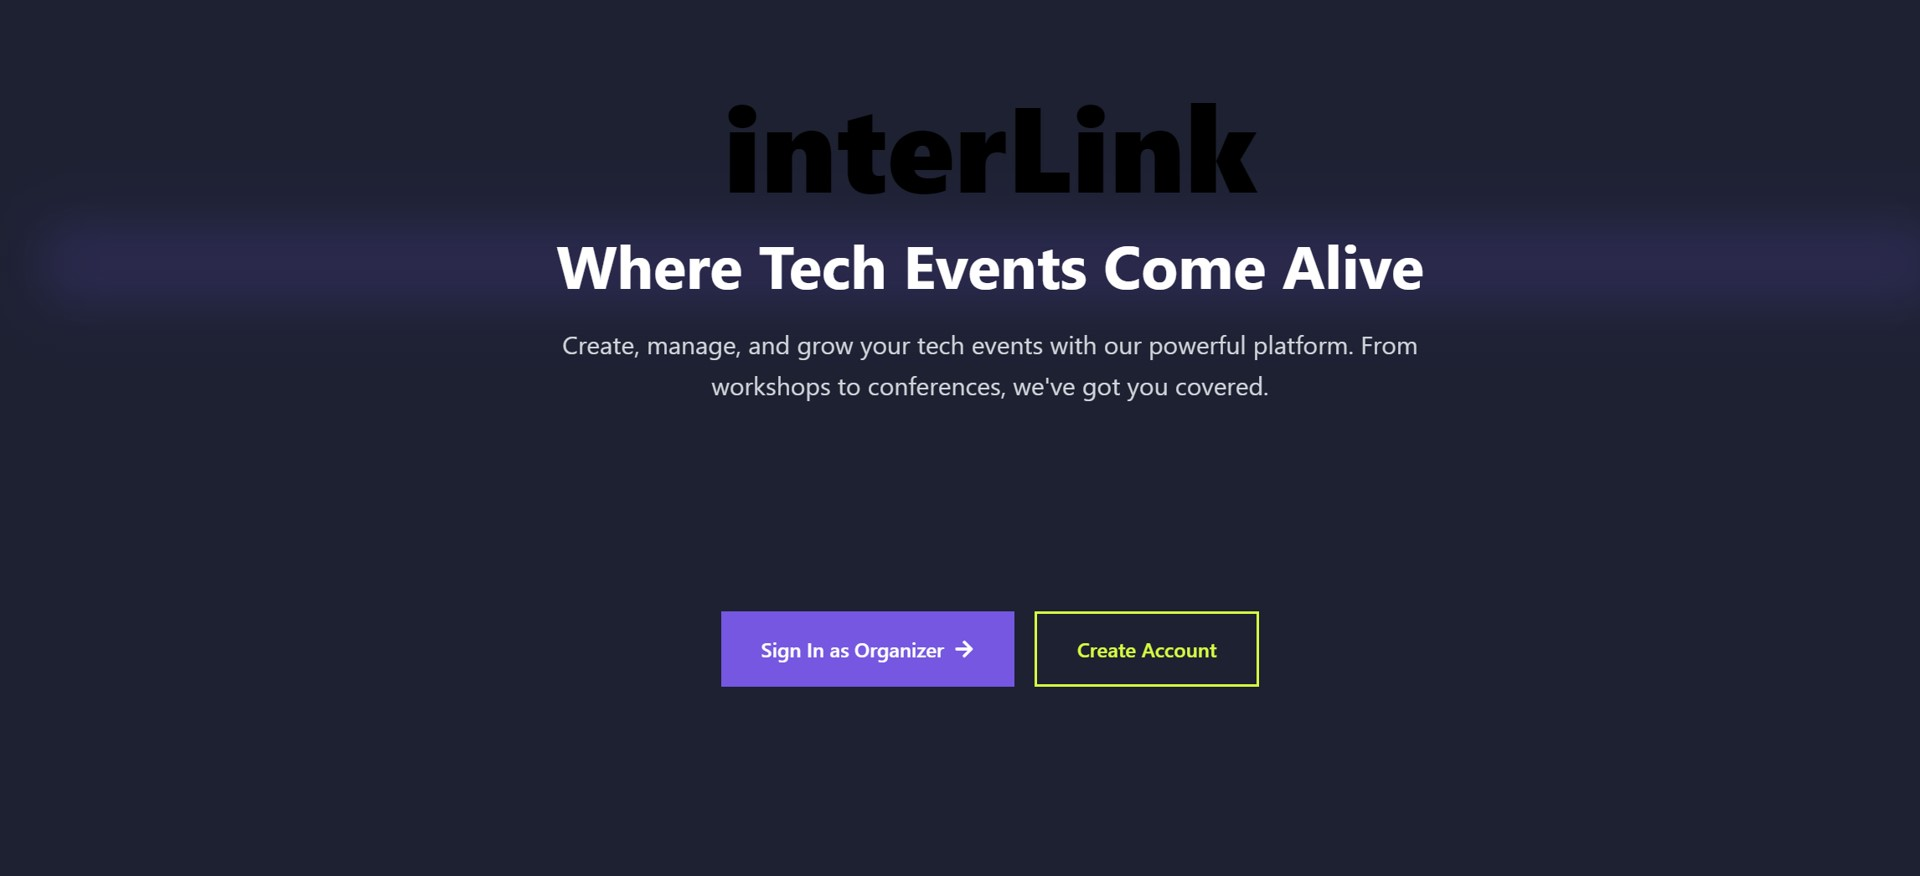
\includegraphics[scale=0.35]{r6.jpg}
		\caption{Organizer Home } % Description above the image     
	\end{figure}
	
	\begin{figure}[H]
		\centering
		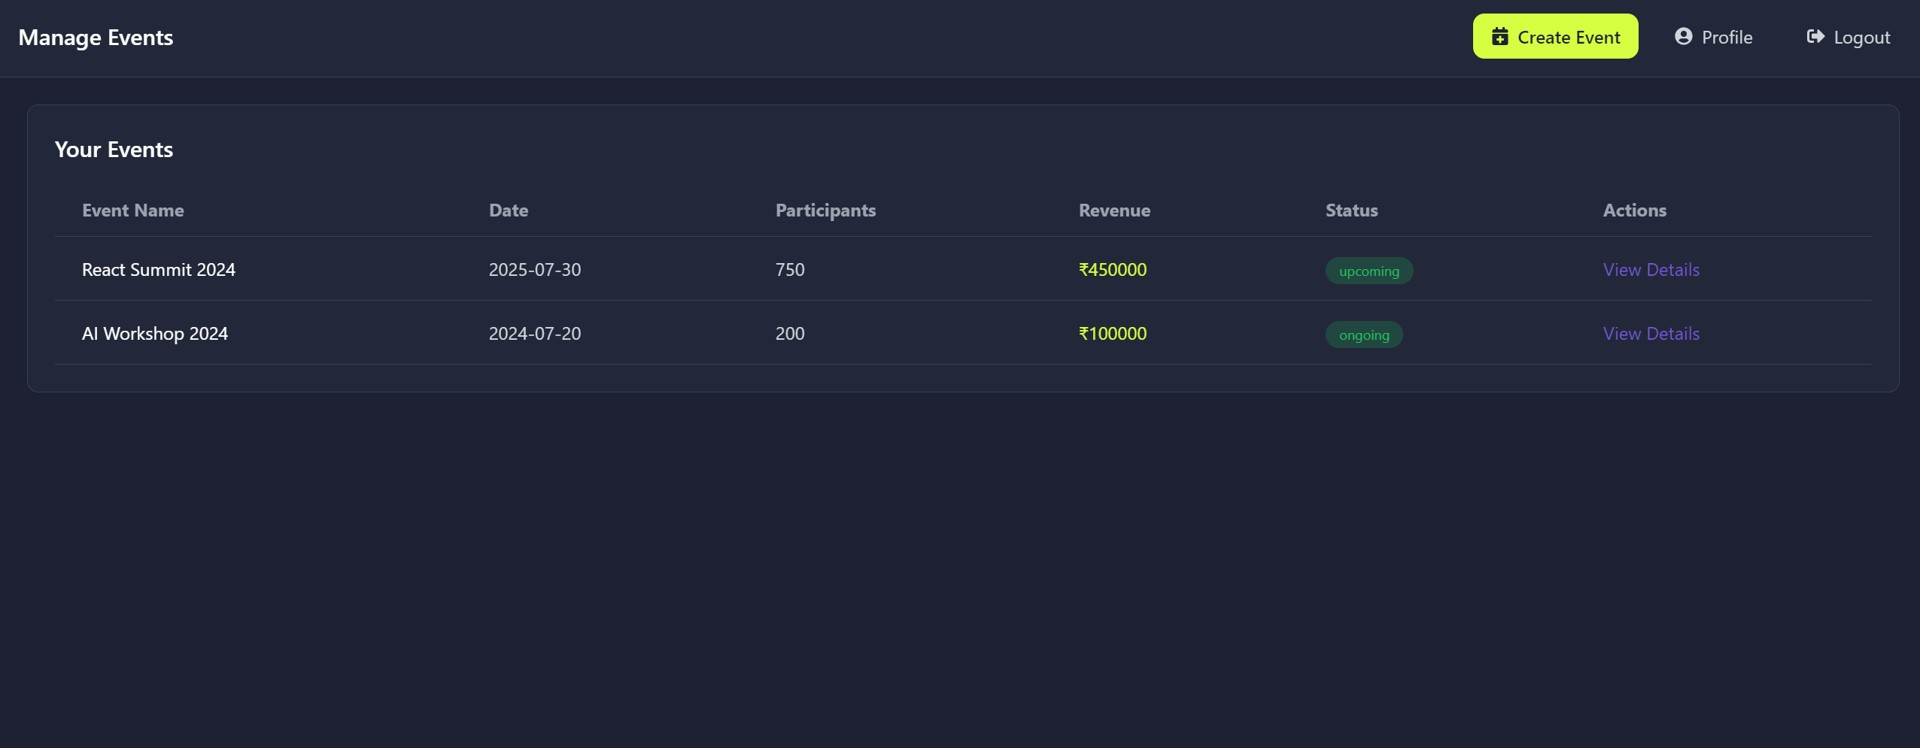
\includegraphics[scale=0.35]{r7.jpg}
		\caption{Organizer Dashboard} % Description above the image     
	\end{figure}
	
	\begin{figure}[H]
		\centering
		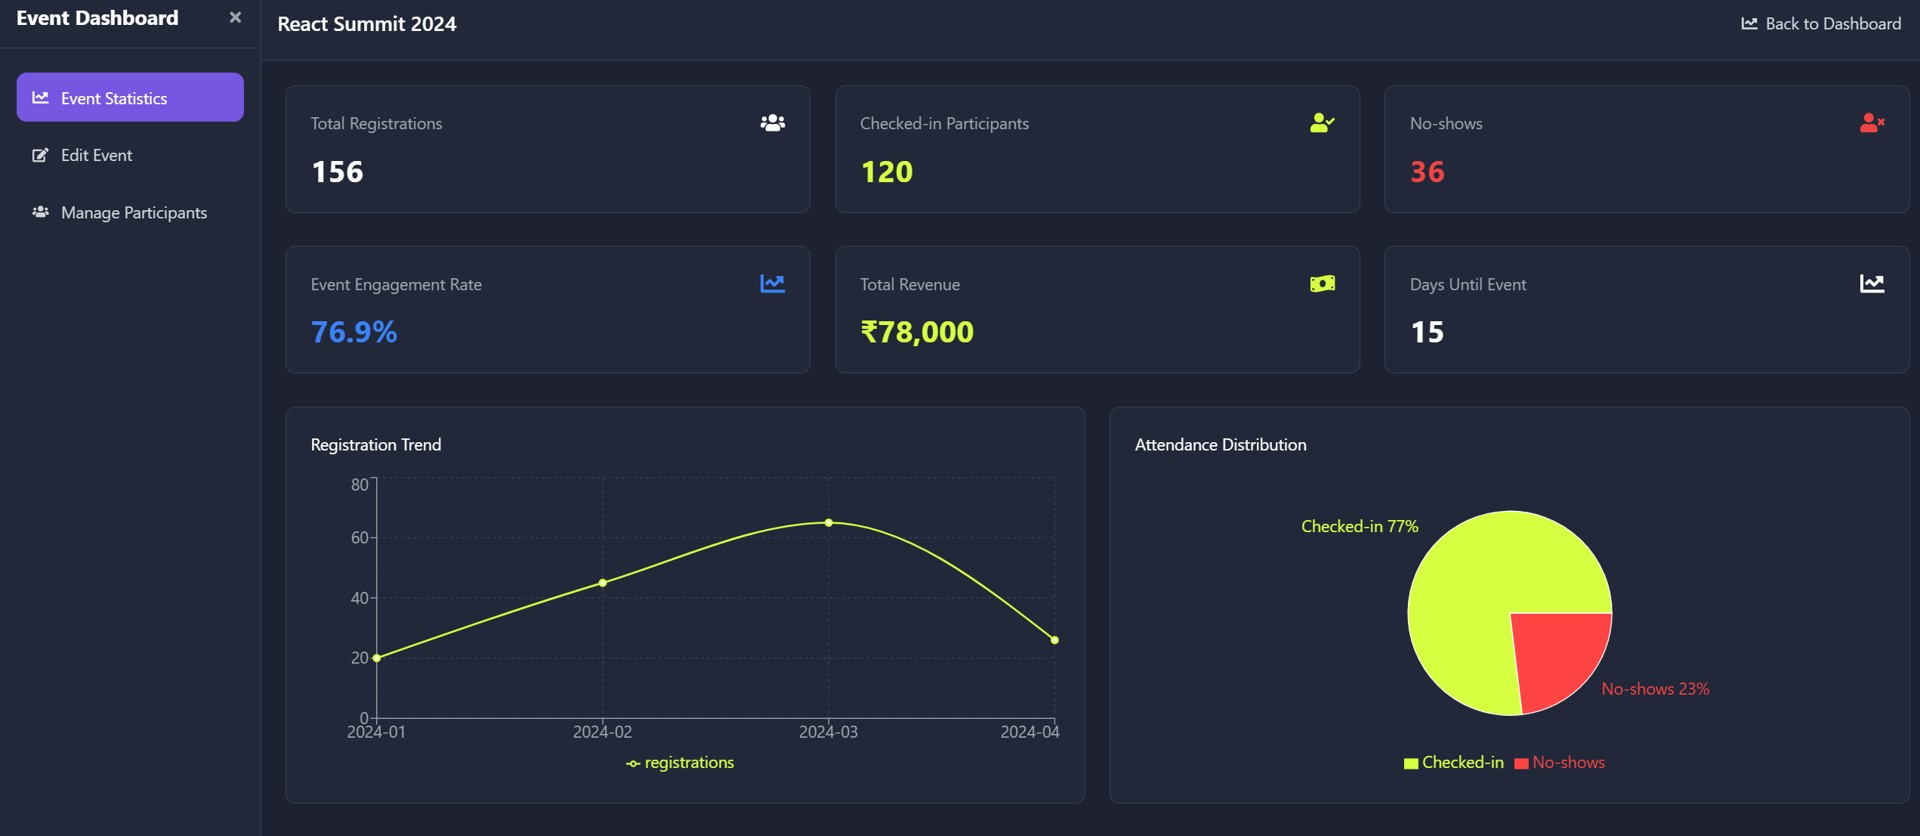
\includegraphics[scale=0.35]{r8.jpg}   
		\caption{Organizer Event Dashboard} % Description above the image  
	\end{figure}
	
	\begin{figure}[H]
		\centering
		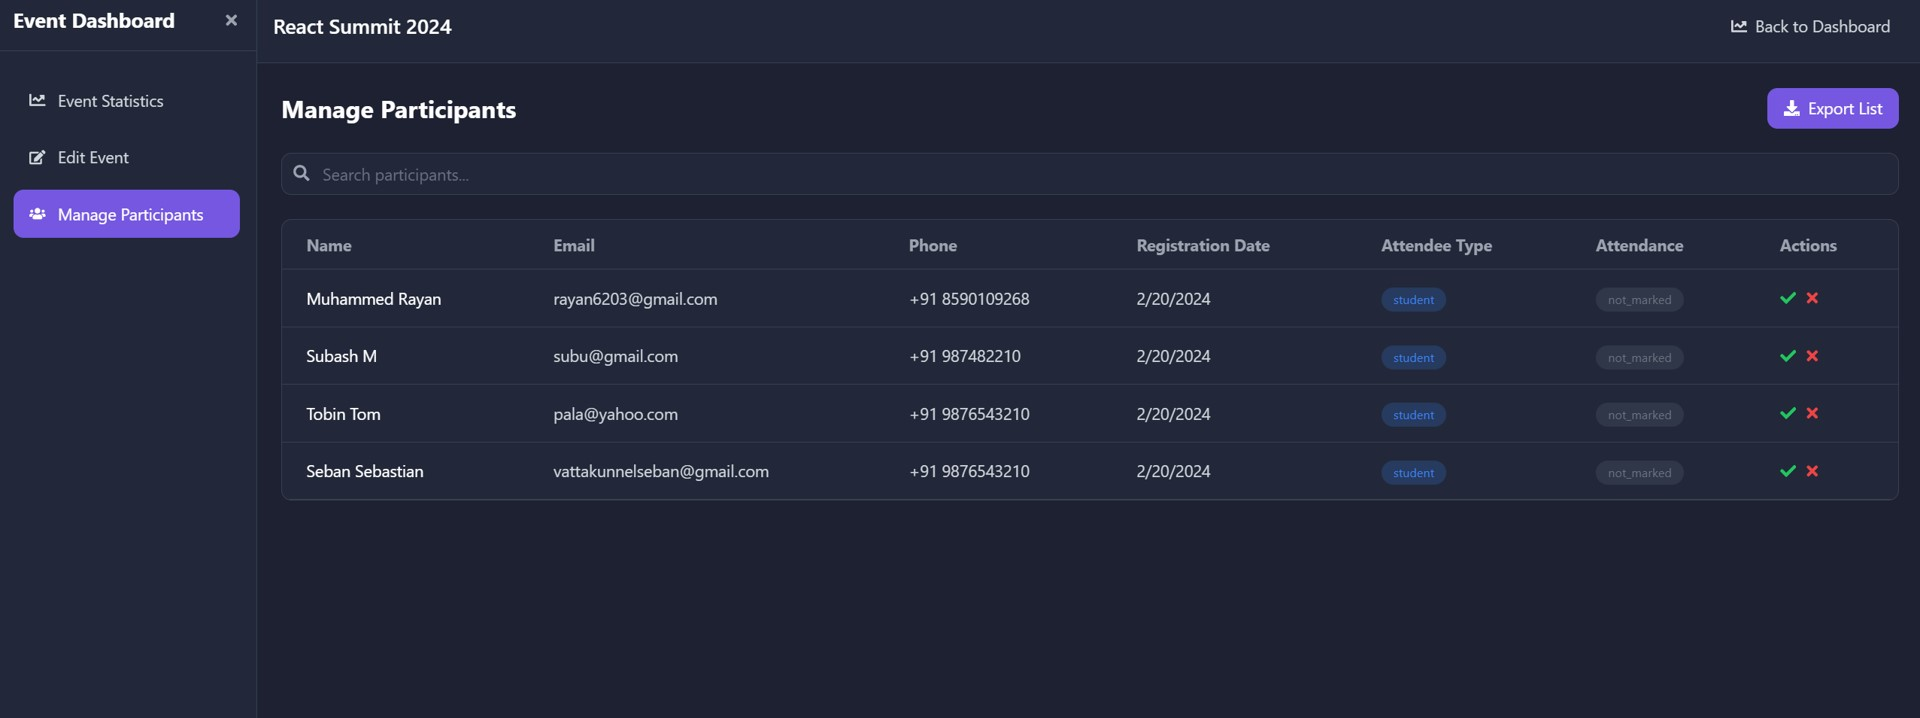
\includegraphics[scale=0.35]{r9.jpg}   
		\caption{Organizer Event Dashboard – Manage Particpants} % Description above the image  
	\end{figure}
	
\end{flushleft}
\section {Database Design}


\subsection { ER Diagram}
\vspace{2.40cm}
\begin{flushleft}
	\begin{minipage}{\linewidth}
		\centering
		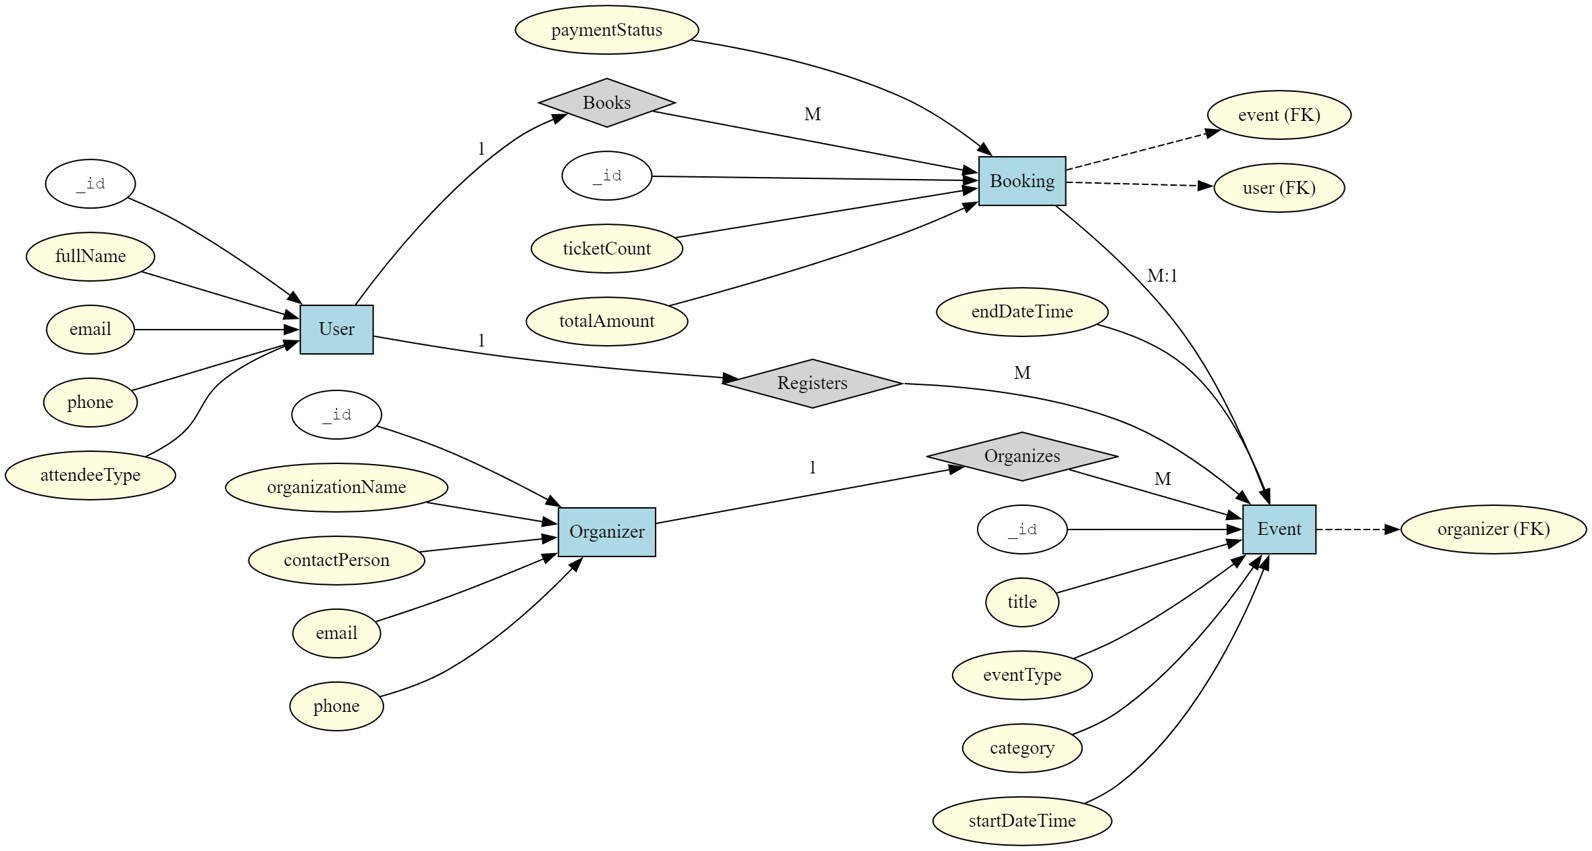
\includegraphics[width=\linewidth]{er.jpg}
	     	\label{fig:er-diagram}
	\end{minipage}
\end{flushleft}
\newpage
\subsection{Tables}

\begin{figure}[ht]
	\centering
	\begin{minipage}{0.45\textwidth}
		\centering
		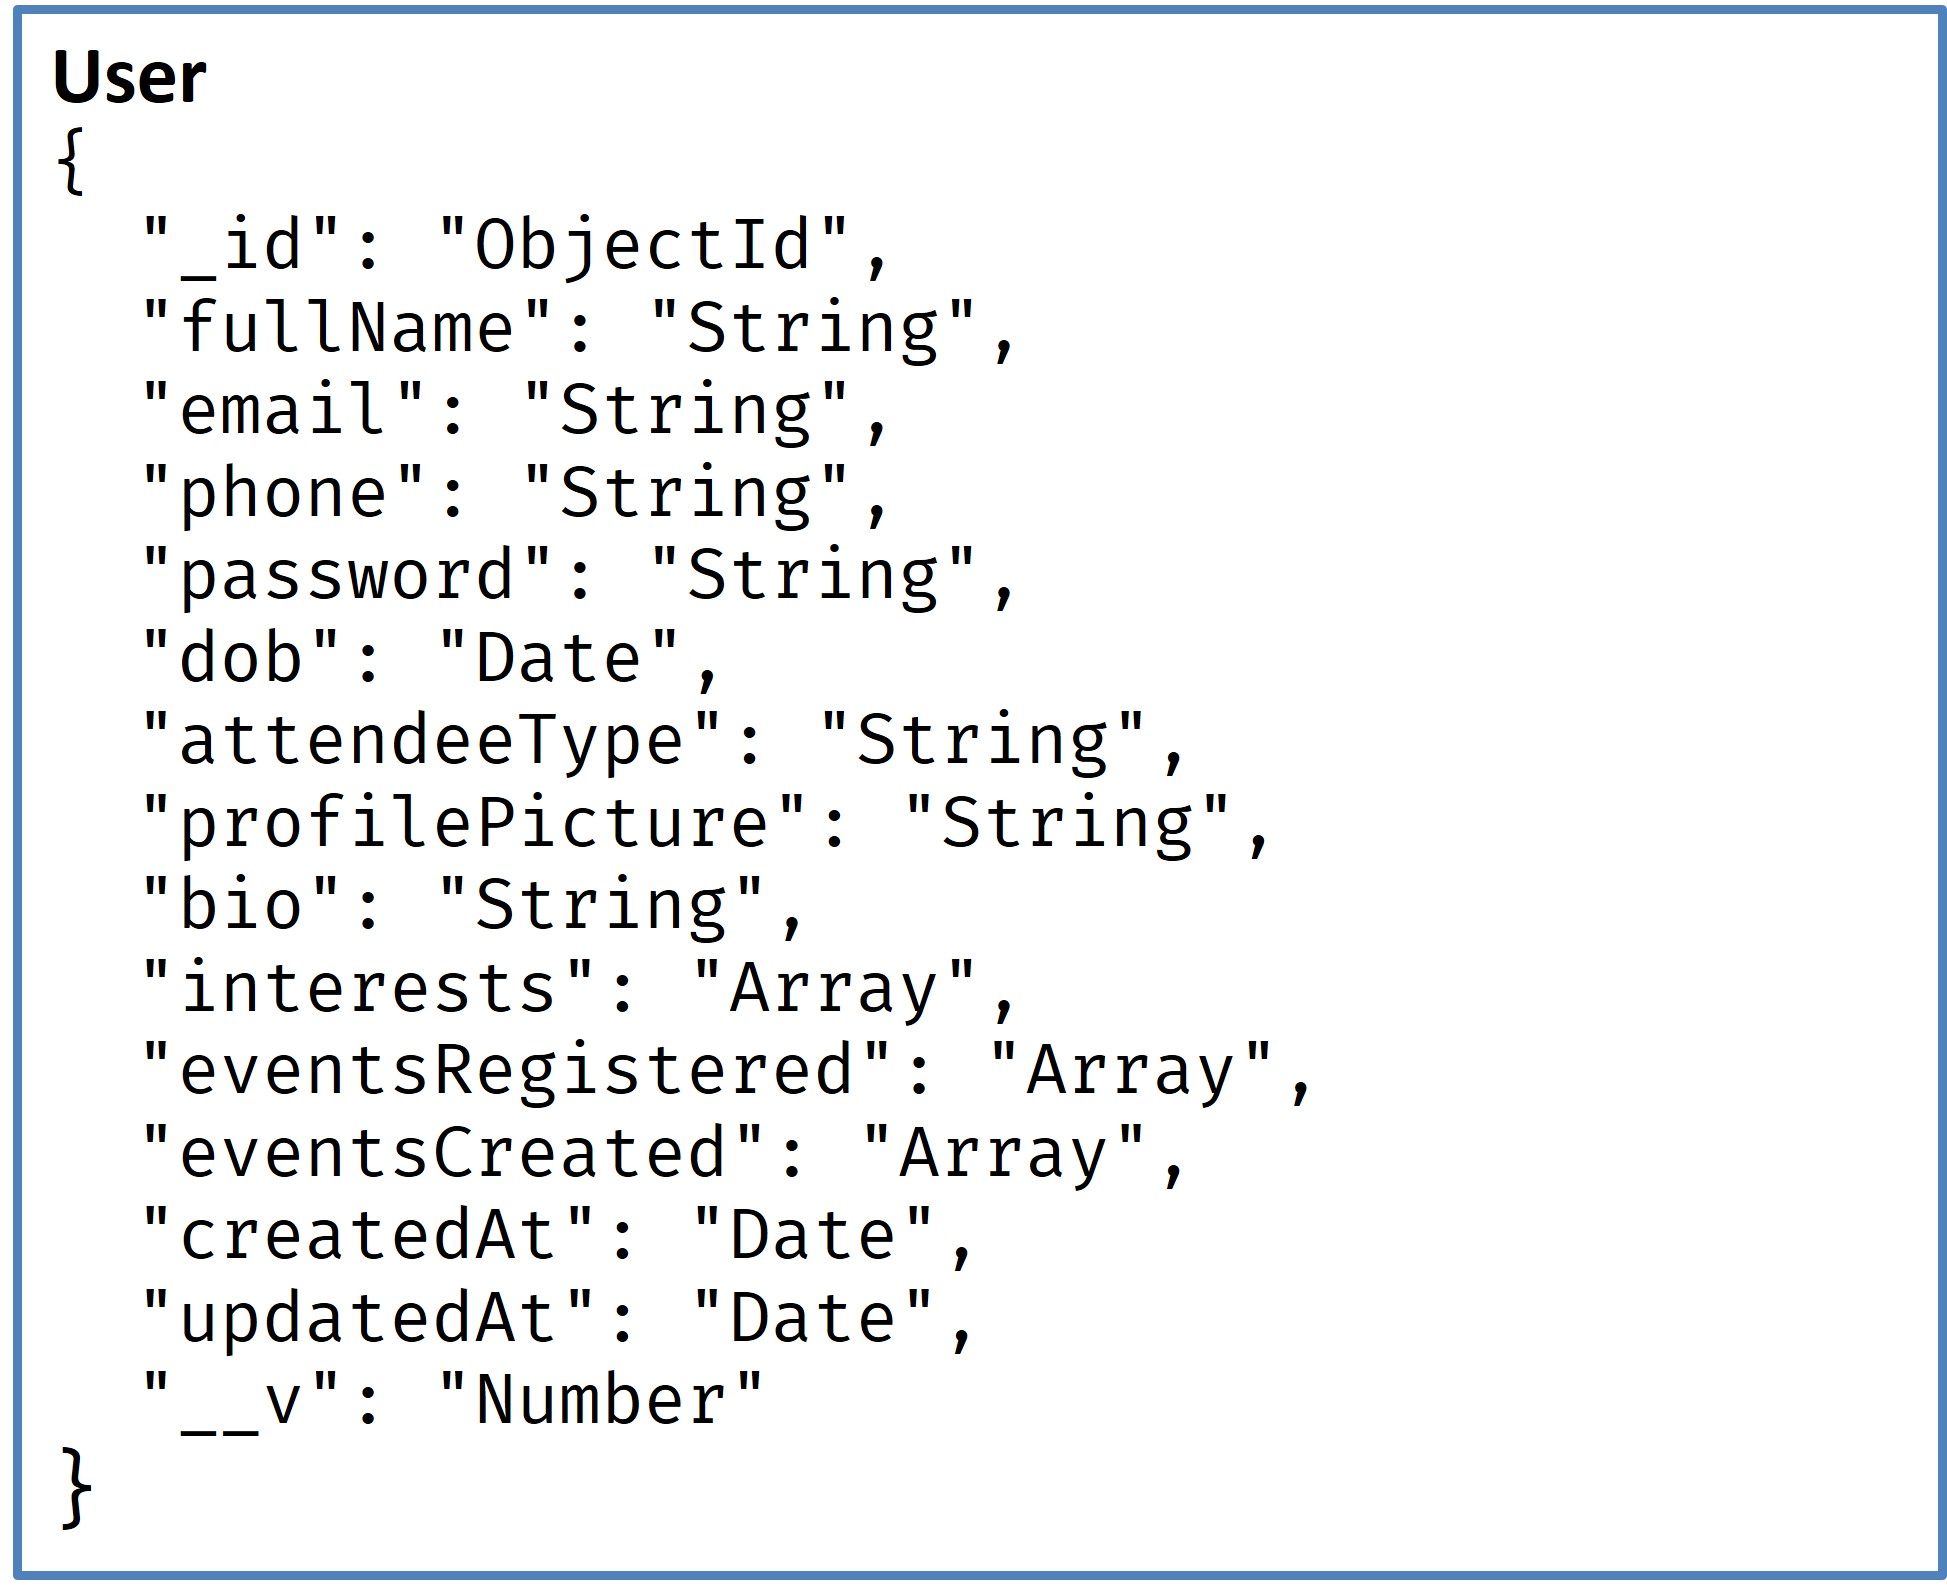
\includegraphics[scale=0.45]{table1.jpg}     
	\end{minipage}\hfill
	\begin{minipage}{0.45\textwidth}
		\centering
		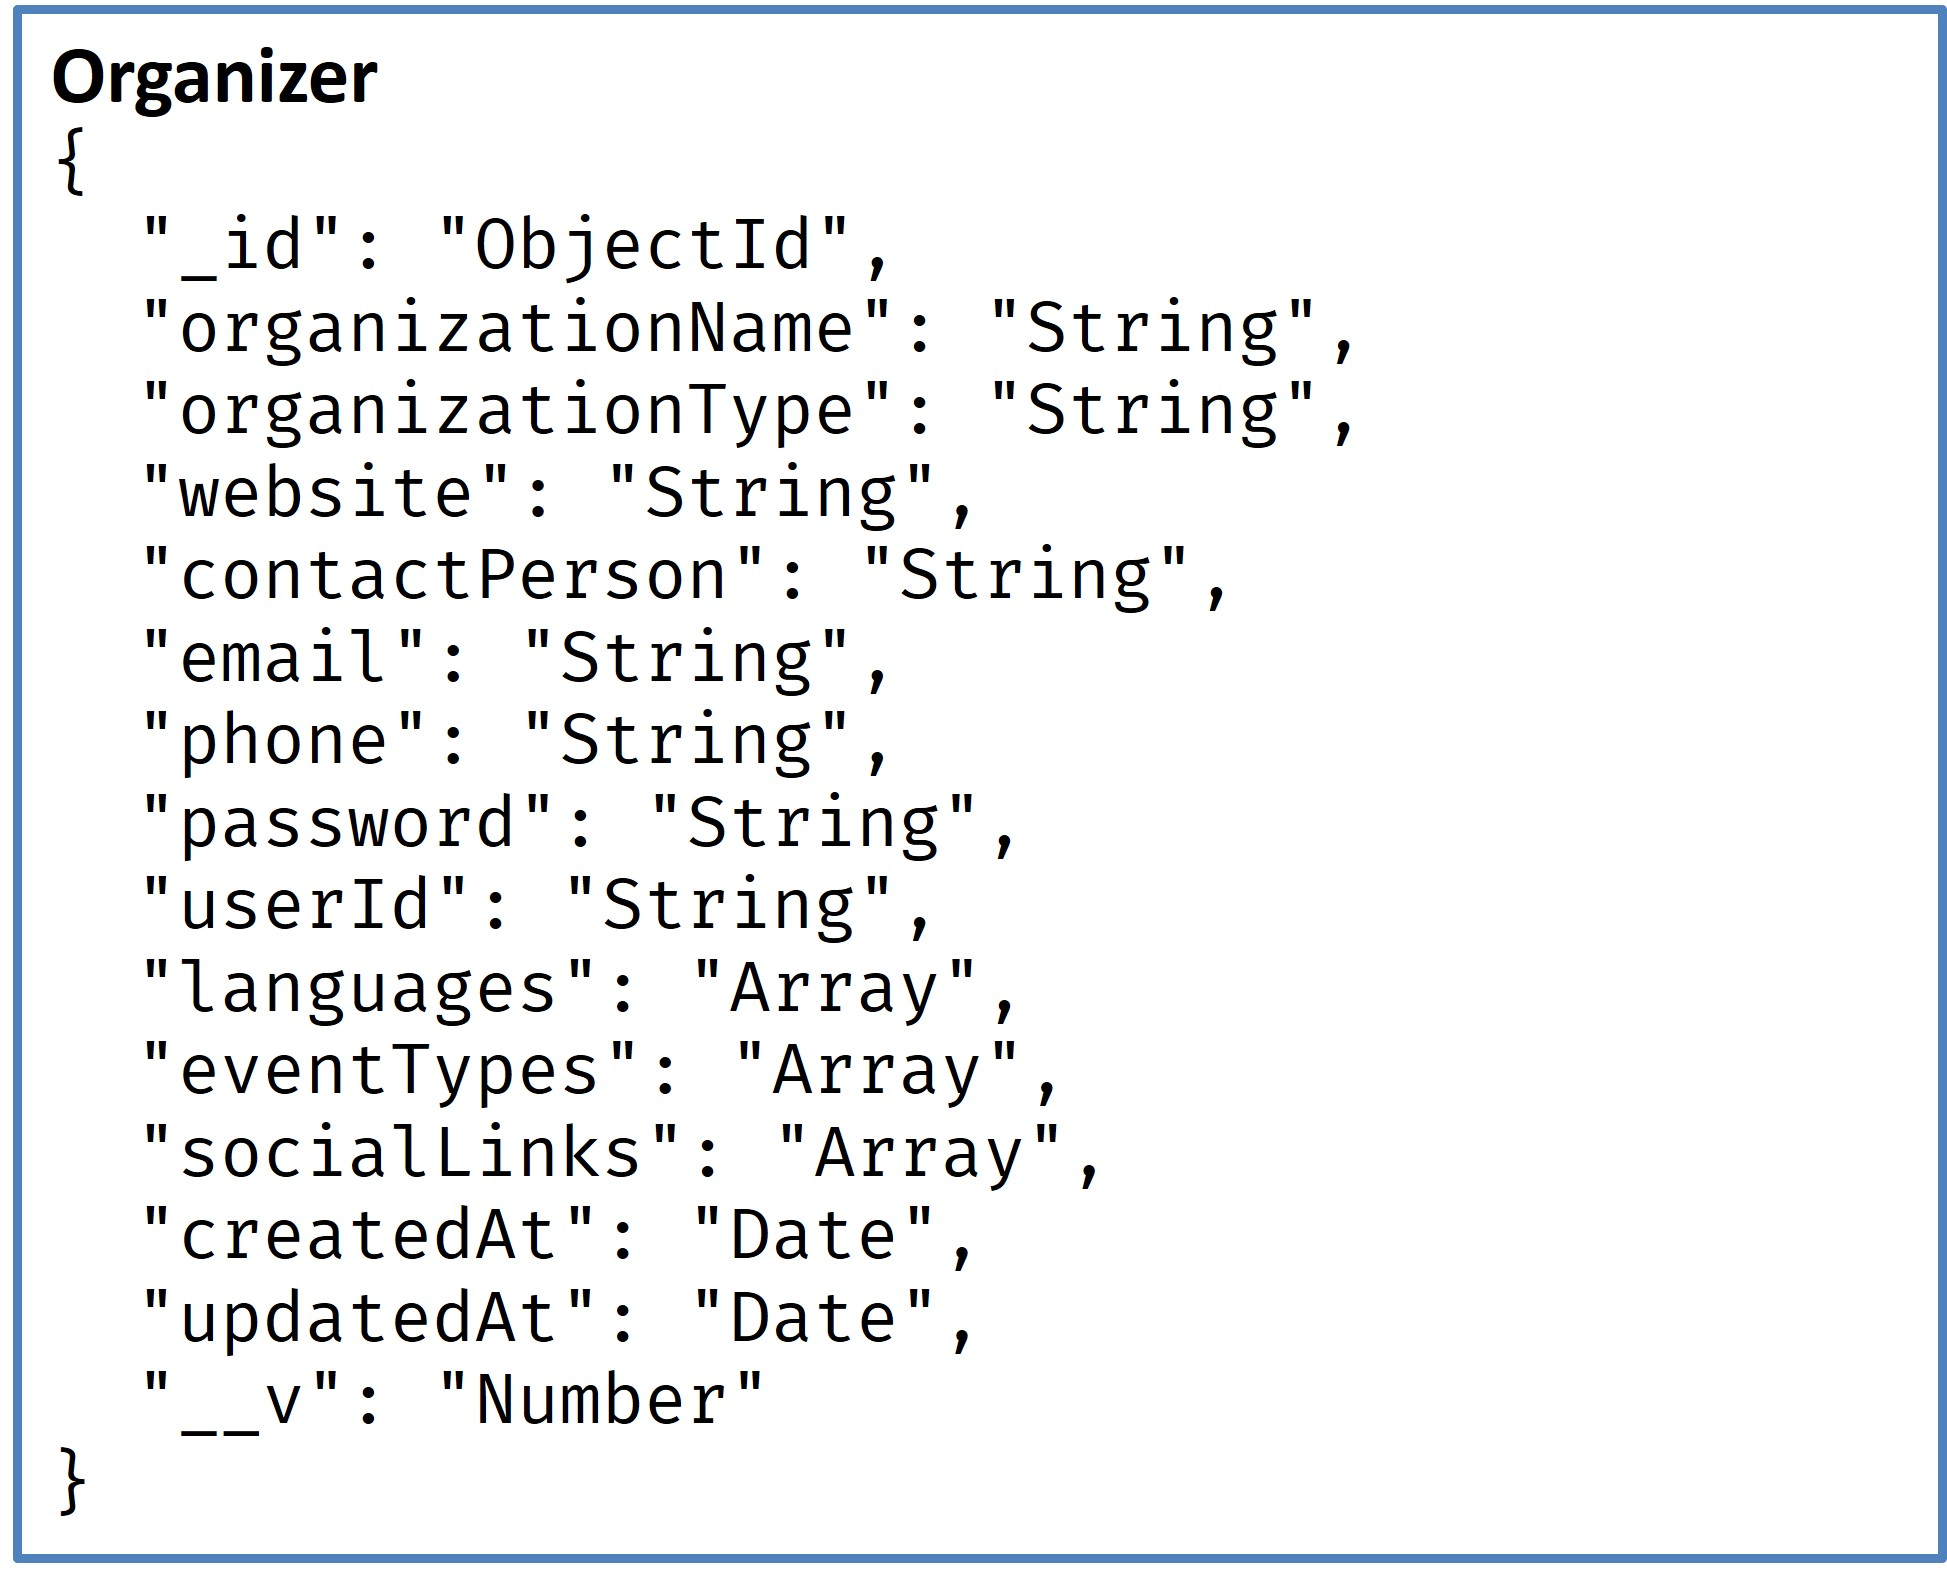
\includegraphics[scale=0.45]{table2.jpg}     
	\end{minipage}
	
	\vspace{1cm} % Adds some vertical space between the rows of images
	
	\begin{minipage}{0.45\textwidth}
		\centering
		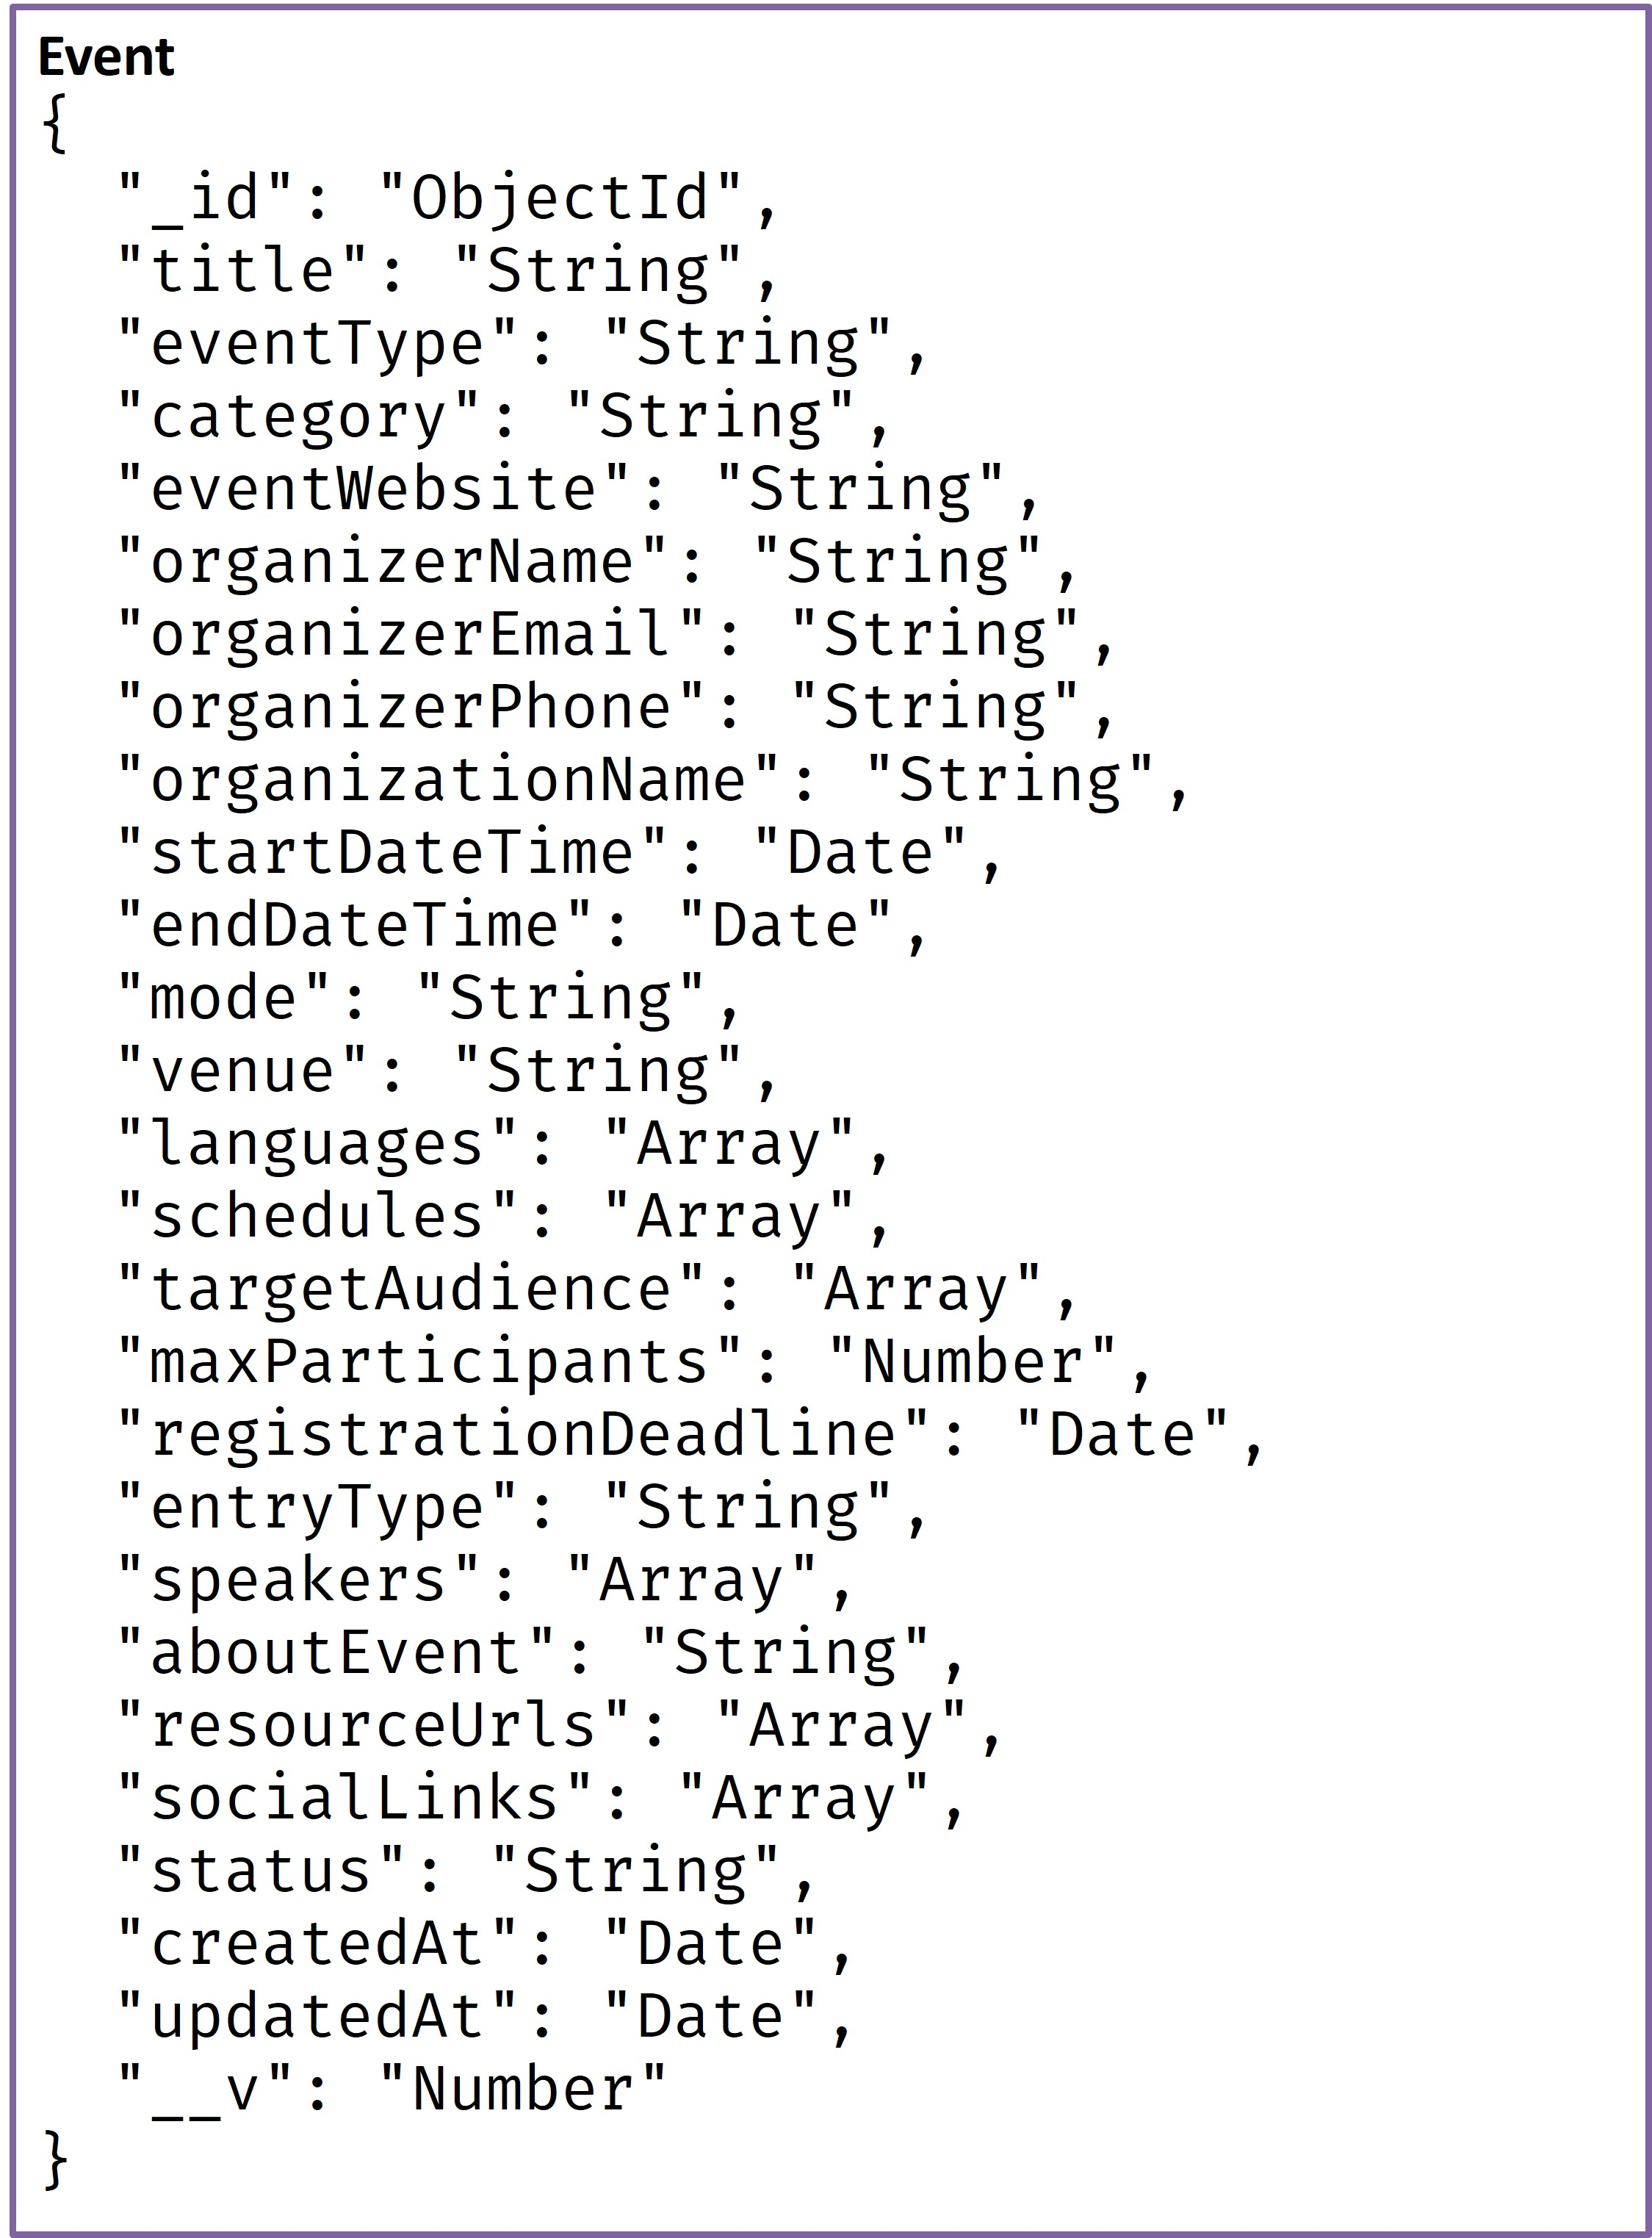
\includegraphics[scale=0.45]{table3.jpg}     
	\end{minipage}\hfill
	\begin{minipage}{0.45\textwidth}
		\centering
		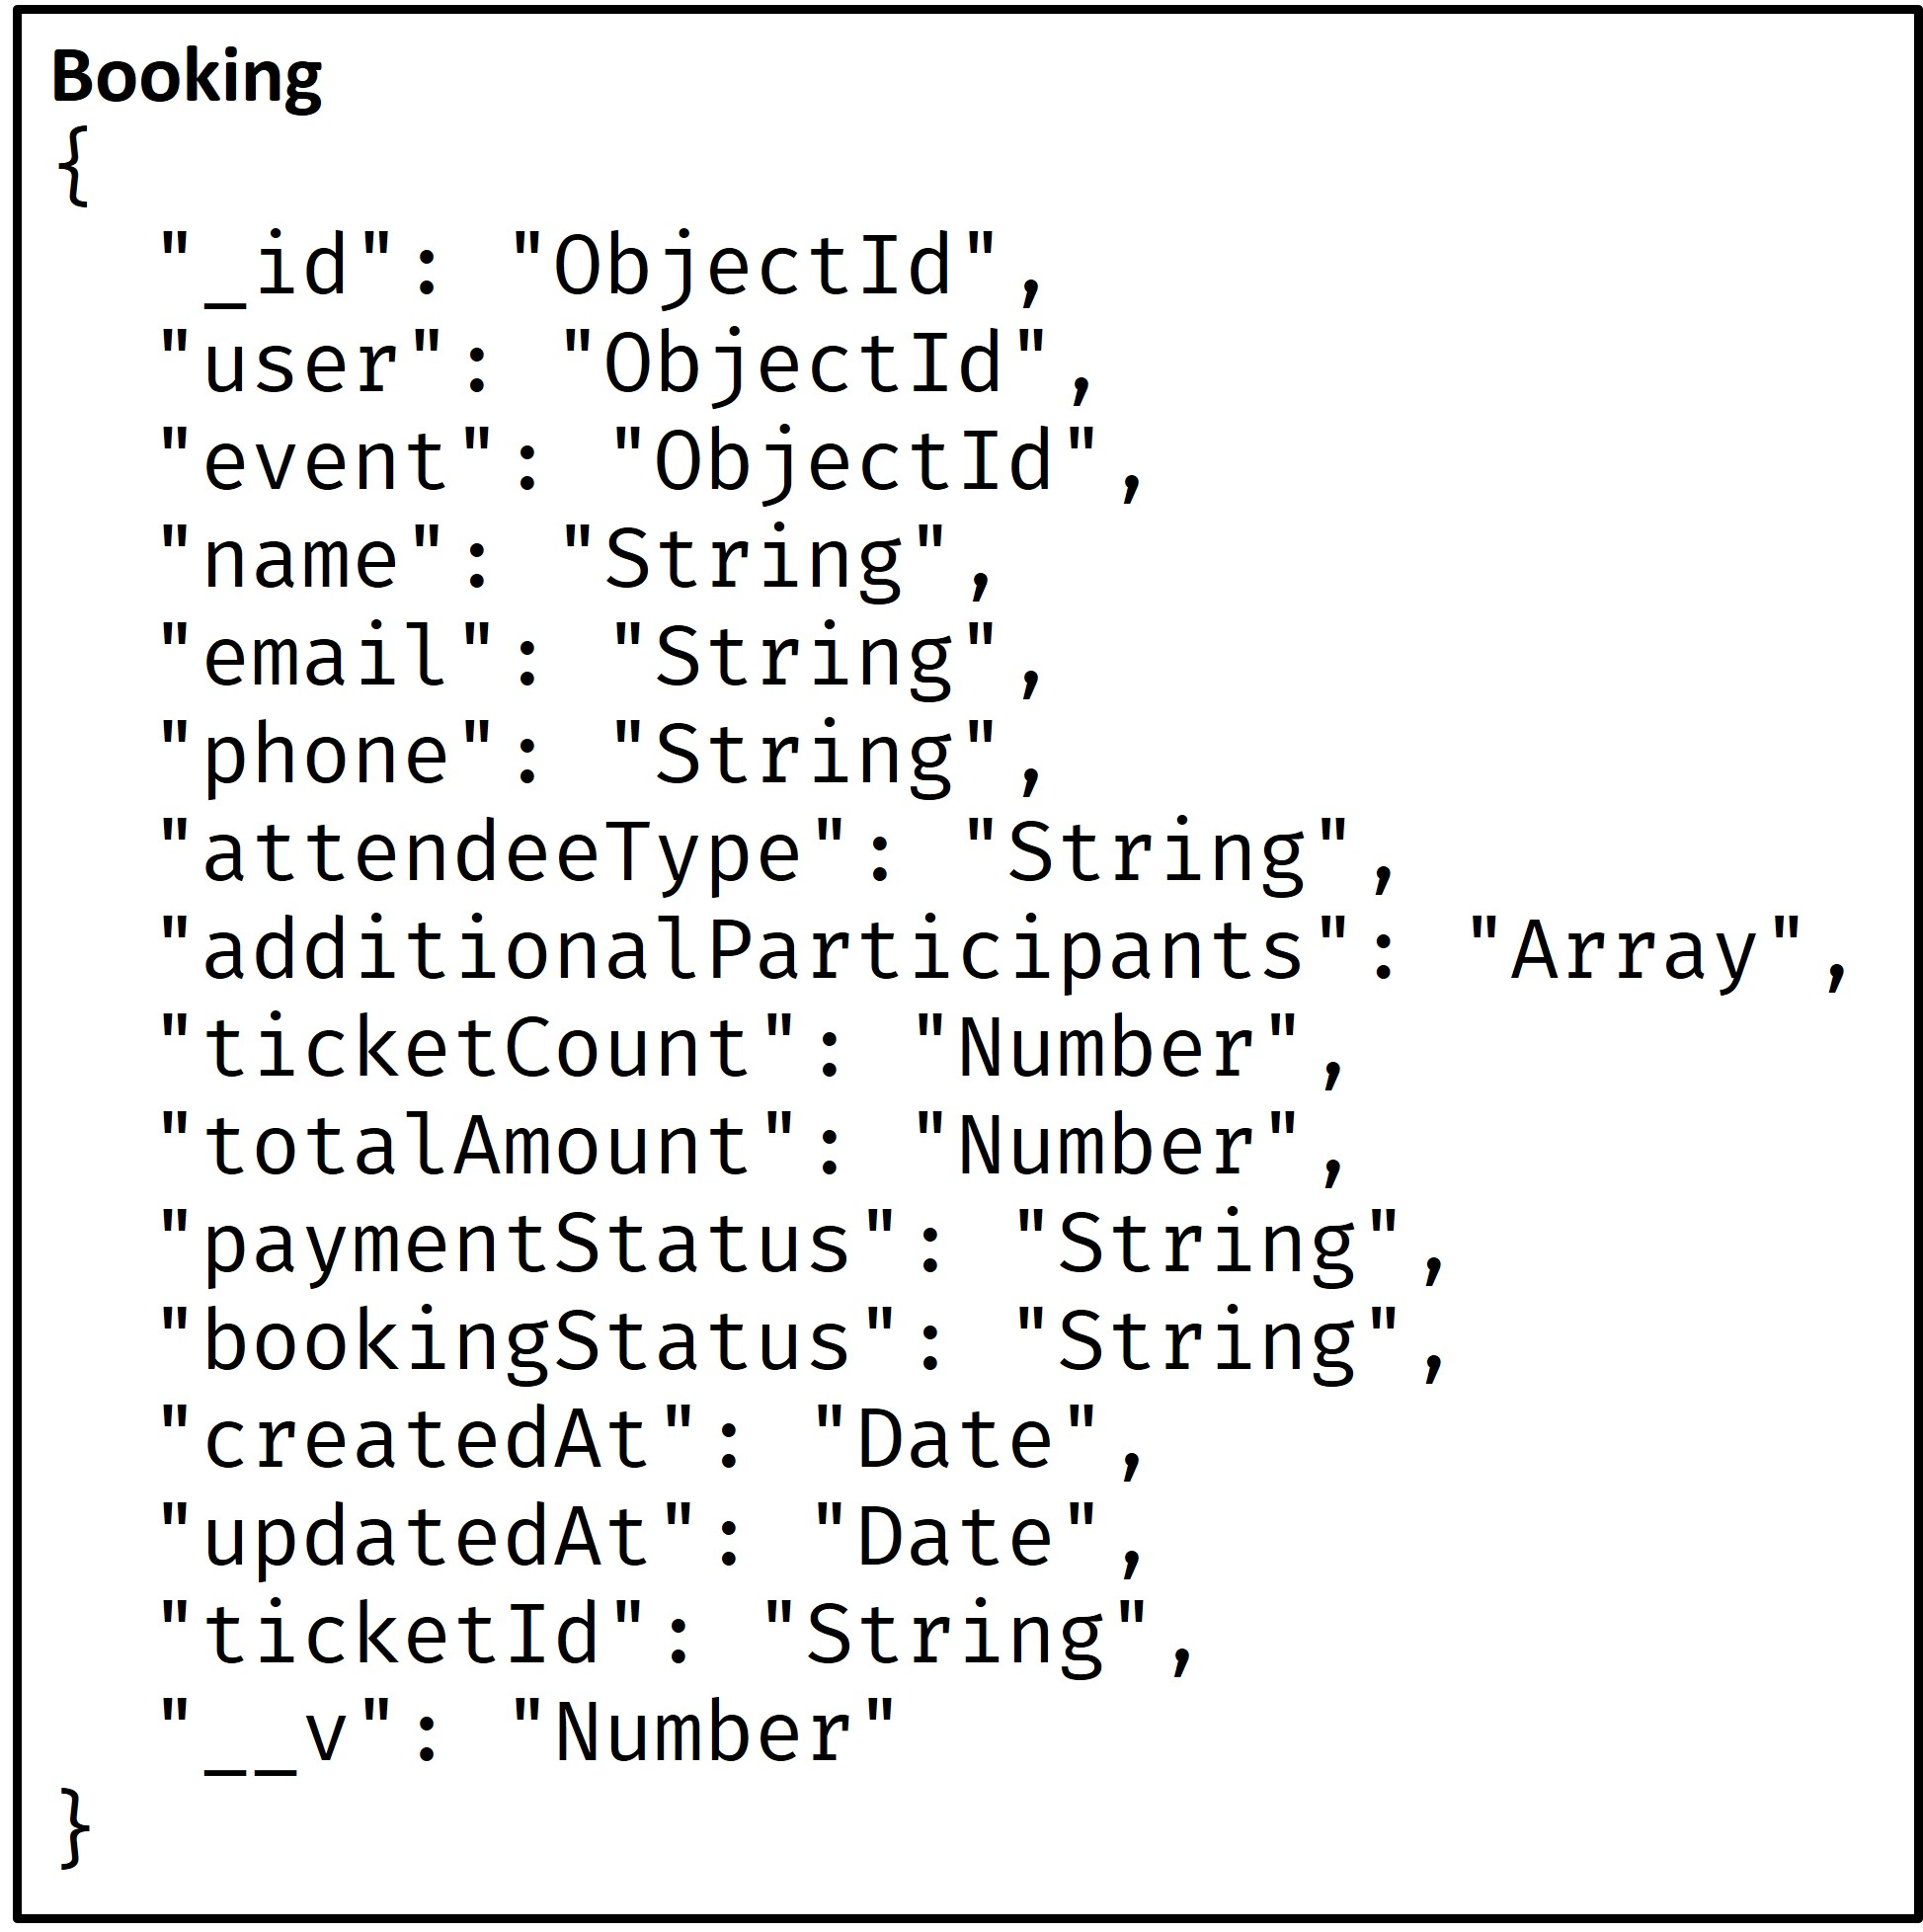
\includegraphics[scale=0.45]{table4.jpg}     
	\end{minipage}
\end{figure}









\begin{flushleft}
	\chapter{System Implementation }
\end{flushleft}
\paragraph{}
\hspace{1.5cm}
The Project has been developed using React.js for front-end and Mongodb for back-end. The project is implemented using React framework, which makes it easy to create interactive and dynamic event booking and publishing system
\section{Modules}
\hspace{1.5cm}
Project has been mainly divided into three modules.
\newline \textbf{Module 1 : User Authentication and Authorization Module}
\begin{itemize}
	\item Manages user registration, login, and JWT token generation for session management.
	\item Ensures role-based access (Viewer/Publisher) for different functionalities.
\end{itemize}
\textbf{Module 2 : Event Management Module (Publisher)}
\begin{itemize}
	\item Allows publishers to create, edit, and manage events with detailed information.
	\item Tracks bookings, available seats, and provides event analytics.
\end{itemize}
%\newpage
\textbf{Module 3 :Event Browsing and Booking Module(Viewer)}
\begin{itemize}
	\item Viewers can browse, search, and filter events by categories like location and date.
	\item Allows viewers to book tickets and manage their booking history.
\end{itemize}
\textbf{Module 4 :Booking Management Module)}
\begin{itemize}
	\item Handles ticket booking, ensuring seat availability and confirming bookings.
	\item Manages booking history, including cancellation and updates.
\end{itemize}
\textbf{Module 4 :Payment Gateway Integration Module)}
\begin{itemize}
	\item Integrates with third-party services (e.g., Stripe, PayPal) to process payments for event bookings.
	\item Manages payment confirmations, secure transactions, and refunds if needed.
\end{itemize}























\begin{flushleft}
	\chapter{Conclusion and Future Scope}
\end{flushleft}
%\end{flushleft}
\paragraph{}
\hspace{1.5cm}
\justify
This platform provides a comprehensive solution for both event organizers and participants, streamlining event management and enhancing accessibility. It offers a user-friendly interface for browsing, booking, and managing events, while organizers can efficiently publish, track bookings, and manage event details. Key features like robust user management, secure payment integration, and intuitive dashboards make it a scalable platform that meets the diverse needs of the community, fostering collaboration and efficient event experiences.

\paragraph{}
\hspace{1.5cm}
Looking ahead, the platform has significant potential for growth. Future enhancements could include mobile app integration, personalized event recommendations, real-time notifications, and expanded payment options to improve accessibility and user engagement. Additionally, adding multilingual support, detailed analytics for organizers, and social media integration could help broaden the platform’s reach, ensuring it remains adaptable and efficient for a global audience.
%\pagestyle{empty}












%\pagestyle{empty}
%\begin{flushleft}
\newpage
\nocite{*}
\addcontentsline{toc}{chapter}{Bibliography}
\bibliographystyle{plain}
\bibliography{reference.bib}
\end{document}
